\documentclass{book}
\usepackage[a4paper,top=2.5cm,bottom=2.5cm,left=2.5cm,right=2.5cm]{geometry}
\usepackage{makeidx}
\usepackage{natbib}
\usepackage{graphicx}
\usepackage{multicol}
\usepackage{float}
\usepackage{listings}
\usepackage{color}
\usepackage{ifthen}
\usepackage[table]{xcolor}
\usepackage{textcomp}
\usepackage{alltt}
\usepackage{ifpdf}
\ifpdf
\usepackage[pdftex,
            pagebackref=true,
            colorlinks=true,
            linkcolor=blue,
            unicode
           ]{hyperref}
\else
\usepackage[ps2pdf,
            pagebackref=true,
            colorlinks=true,
            linkcolor=blue,
            unicode
           ]{hyperref}
\usepackage{pspicture}
\fi
\usepackage[utf8]{inputenc}
\usepackage{mathptmx}
\usepackage[scaled=.90]{helvet}
\usepackage{courier}
\usepackage{sectsty}
\usepackage{amssymb}
\usepackage[titles]{tocloft}
\usepackage{doxygen}
\lstset{language=C++,inputencoding=utf8,basicstyle=\footnotesize,breaklines=true,breakatwhitespace=true,tabsize=4,numbers=left }
\makeindex
\setcounter{tocdepth}{3}
\renewcommand{\footrulewidth}{0.4pt}
\renewcommand{\familydefault}{\sfdefault}
\hfuzz=15pt
\setlength{\emergencystretch}{15pt}
\hbadness=750
\tolerance=750
\begin{document}
\hypersetup{pageanchor=false,citecolor=blue}
\begin{titlepage}
\vspace*{7cm}
\begin{center}
{\Large Creative Evolution Tools \\[1ex]\large 0.\-1.\-0 }\\
\vspace*{1cm}
{\large Generated by Doxygen 1.8.3.1}\\
\vspace*{0.5cm}
{\small Mon Nov 4 2013 15:38:37}\\
\end{center}
\end{titlepage}
\clearemptydoublepage
\pagenumbering{roman}
\tableofcontents
\clearemptydoublepage
\pagenumbering{arabic}
\hypersetup{pageanchor=true,citecolor=blue}
\chapter{Hierarchical Index}
\section{Class Hierarchy}
This inheritance list is sorted roughly, but not completely, alphabetically\-:\begin{DoxyCompactList}
\item \contentsline{section}{Assertion}{\pageref{class_assertion}}{}
\item \contentsline{section}{Assertion\-Group}{\pageref{class_assertion_group}}{}
\item \contentsline{section}{Font\-Family}{\pageref{class_font_family}}{}
\item \contentsline{section}{Font\-Family\-Node}{\pageref{class_font_family_node}}{}
\item \contentsline{section}{Font\-Suitcase}{\pageref{class_font_suitcase}}{}
\item \contentsline{section}{Gui\-Base}{\pageref{class_gui_base}}{}
\begin{DoxyCompactList}
\item \contentsline{section}{Gui\-Rect}{\pageref{class_gui_rect}}{}
\begin{DoxyCompactList}
\item \contentsline{section}{Gui\-Plot}{\pageref{class_gui_plot}}{}
\end{DoxyCompactList}
\item \contentsline{section}{Gui\-Text}{\pageref{class_gui_text}}{}
\end{DoxyCompactList}
\item \contentsline{section}{Plotter\-Data}{\pageref{class_plotter_data}}{}
\begin{DoxyCompactList}
\item \contentsline{section}{Poly\-Line\-Data}{\pageref{class_poly_line_data}}{}
\item \contentsline{section}{Polynomial\-Data}{\pageref{class_polynomial_data}}{}
\end{DoxyCompactList}
\item \contentsline{section}{Polynomial\-Population}{\pageref{class_polynomial_population}}{}
\end{DoxyCompactList}

\chapter{Class Index}
\section{Class List}
Here are the classes, structs, unions and interfaces with brief descriptions\-:\begin{DoxyCompactList}
\item\contentsline{section}{\hyperlink{class_assertion}{Assertion} \\*A compact description of a comparative assertion template }{\pageref{class_assertion}}{}
\item\contentsline{section}{\hyperlink{class_assertion_group}{Assertion\-Group} \\*A wrapper class for a group of \hyperlink{class_assertion}{Assertion} items }{\pageref{class_assertion_group}}{}
\item\contentsline{section}{\hyperlink{class_font_family}{Font\-Family} \\*A wrapper for a gl\-::\-Texture\-Font family }{\pageref{class_font_family}}{}
\item\contentsline{section}{\hyperlink{class_font_family_node}{Font\-Family\-Node} \\*A wrapper for a gl\-::\-Texture\-Font node }{\pageref{class_font_family_node}}{}
\item\contentsline{section}{\hyperlink{class_font_suitcase}{Font\-Suitcase} \\*A wrapper for a collection of gl\-::\-Texture\-Font families }{\pageref{class_font_suitcase}}{}
\item\contentsline{section}{\hyperlink{class_gui_base}{Gui\-Base} \\*A basic two-\/dimensional scenegraph node }{\pageref{class_gui_base}}{}
\item\contentsline{section}{\hyperlink{class_gui_plot}{Gui\-Plot} \\*A 2\-D plotting widget }{\pageref{class_gui_plot}}{}
\item\contentsline{section}{\hyperlink{class_gui_rect}{Gui\-Rect} \\*A scenegraph node representing a rectangle }{\pageref{class_gui_rect}}{}
\item\contentsline{section}{\hyperlink{class_gui_text}{Gui\-Text} \\*A scenegraph node representing a text label }{\pageref{class_gui_text}}{}
\item\contentsline{section}{\hyperlink{class_plotter_data}{Plotter\-Data} \\*Base class representing data to be plotted by \hyperlink{class_gui_plot}{Gui\-Plot} }{\pageref{class_plotter_data}}{}
\item\contentsline{section}{\hyperlink{class_poly_line_data}{Poly\-Line\-Data} \\*Implements a subclass of \hyperlink{class_plotter_data}{Plotter\-Data} that stores ci\-::\-Poly\-Line2f data }{\pageref{class_poly_line_data}}{}
\item\contentsline{section}{\hyperlink{class_polynomial_data}{Polynomial\-Data} \\*A class representing a polynomial function }{\pageref{class_polynomial_data}}{}
\item\contentsline{section}{\hyperlink{class_polynomial_population}{Polynomial\-Population} \\*A population container and evolutionary process facilitation class for polynomial data and assertions }{\pageref{class_polynomial_population}}{}
\end{DoxyCompactList}

\chapter{Class Documentation}
\hypertarget{class_assertion}{\section{Assertion Class Reference}
\label{class_assertion}\index{Assertion@{Assertion}}
}


A compact description of a comparative assertion template.  




{\ttfamily \#include $<$Polynomial\-Assertion.\-h$>$}

\subsection*{Public Member Functions}
\begin{DoxyCompactItemize}
\item 
\hypertarget{class_assertion_a97bcb911418eb279c6ccc6236208a06a}{\hyperlink{class_assertion_a97bcb911418eb279c6ccc6236208a06a}{Assertion} ()}\label{class_assertion_a97bcb911418eb279c6ccc6236208a06a}

\begin{DoxyCompactList}\small\item\em Default constructor. \end{DoxyCompactList}\item 
\hypertarget{class_assertion_a3acb3e23e1c425d1a017edf3186b31fa}{float \hyperlink{class_assertion_a3acb3e23e1c425d1a017edf3186b31fa}{apply\-To} (Polynomial\-Data\-Ref i\-Lhs\-Ref) const }\label{class_assertion_a3acb3e23e1c425d1a017edf3186b31fa}

\begin{DoxyCompactList}\small\item\em Applies the assertion to the given left-\/hand data. \end{DoxyCompactList}\item 
\hypertarget{class_assertion_a8181e04370c4581826e2d93973373def}{std\-::string \hyperlink{class_assertion_a8181e04370c4581826e2d93973373def}{get\-Assertion\-String} (Polynomial\-Data\-Ref i\-Lhs\-Ref) const }\label{class_assertion_a8181e04370c4581826e2d93973373def}

\begin{DoxyCompactList}\small\item\em Returns a formatted string representing the assertion. \end{DoxyCompactList}\item 
\hypertarget{class_assertion_a32800847872df8197d7d640584c19592}{void \hyperlink{class_assertion_a32800847872df8197d7d640584c19592}{set\-Data\-Rhs} (Polynomial\-Data\-Ref i\-Data\-Rhs)}\label{class_assertion_a32800847872df8197d7d640584c19592}

\begin{DoxyCompactList}\small\item\em Sets the right-\/hand data reference. \end{DoxyCompactList}\item 
\hypertarget{class_assertion_a0daf687650609e4629d06418152a1985}{Polynomial\-Data\-Ref \hyperlink{class_assertion_a0daf687650609e4629d06418152a1985}{get\-Data\-Rhs} () const }\label{class_assertion_a0daf687650609e4629d06418152a1985}

\begin{DoxyCompactList}\small\item\em Returns the right-\/hand data reference. \end{DoxyCompactList}\item 
\hypertarget{class_assertion_ae761bb8fbc7d1eed09b3a7462139bcb2}{void \hyperlink{class_assertion_ae761bb8fbc7d1eed09b3a7462139bcb2}{set\-Parameter\-Range} (const float \&i\-Param\-In, const float \&i\-Param\-Out)}\label{class_assertion_ae761bb8fbc7d1eed09b3a7462139bcb2}

\begin{DoxyCompactList}\small\item\em Sets the assertion's parameter range. \end{DoxyCompactList}\item 
\hypertarget{class_assertion_a491e7b2bd569988d9e1b3c62ff438a63}{const float \& \hyperlink{class_assertion_a491e7b2bd569988d9e1b3c62ff438a63}{get\-Parameter\-Range\-In} () const }\label{class_assertion_a491e7b2bd569988d9e1b3c62ff438a63}

\begin{DoxyCompactList}\small\item\em Returns the assertion's lower-\/bounds parameter. \end{DoxyCompactList}\item 
\hypertarget{class_assertion_a3c772dd035cea465322b91c8d4629a38}{const float \& \hyperlink{class_assertion_a3c772dd035cea465322b91c8d4629a38}{get\-Parameter\-Range\-Out} () const }\label{class_assertion_a3c772dd035cea465322b91c8d4629a38}

\begin{DoxyCompactList}\small\item\em Returns the assertion's upper-\/bounds parameter. \end{DoxyCompactList}\item 
\hypertarget{class_assertion_a2557fb49a553c4d271abe420e5ea14cd}{void \hyperlink{class_assertion_a2557fb49a553c4d271abe420e5ea14cd}{set\-Score\-Weight} (const float \&i\-Weight)}\label{class_assertion_a2557fb49a553c4d271abe420e5ea14cd}

\begin{DoxyCompactList}\small\item\em Sets the score weighting multiplier. \end{DoxyCompactList}\item 
\hypertarget{class_assertion_ab56b536f685ec371b16dc563283b6bb6}{const float \& \hyperlink{class_assertion_ab56b536f685ec371b16dc563283b6bb6}{get\-Score\-Weight} () const }\label{class_assertion_ab56b536f685ec371b16dc563283b6bb6}

\begin{DoxyCompactList}\small\item\em Returns the score weighting multiplier. \end{DoxyCompactList}\item 
\hypertarget{class_assertion_ad13971eb3844f686fdd7b48459a0949f}{void \hyperlink{class_assertion_ad13971eb3844f686fdd7b48459a0949f}{set\-Type} (const Assert\-Type \&i\-Type)}\label{class_assertion_ad13971eb3844f686fdd7b48459a0949f}

\begin{DoxyCompactList}\small\item\em Sets the assertion type. \end{DoxyCompactList}\item 
\hypertarget{class_assertion_a7f1f97192d8b0c323de25c70bec720bd}{const Assert\-Type \& \hyperlink{class_assertion_a7f1f97192d8b0c323de25c70bec720bd}{get\-Type} () const }\label{class_assertion_a7f1f97192d8b0c323de25c70bec720bd}

\begin{DoxyCompactList}\small\item\em Returns the assertion type. \end{DoxyCompactList}\item 
\hypertarget{class_assertion_a460c09864d8b88fc263cecef3de8b617}{void \hyperlink{class_assertion_a460c09864d8b88fc263cecef3de8b617}{set\-Mode} (const Assert\-Mode \&i\-Mode\-Lhs, const Assert\-Mode \&i\-Mode\-Rhs)}\label{class_assertion_a460c09864d8b88fc263cecef3de8b617}

\begin{DoxyCompactList}\small\item\em Sets the left-\/hand assertion mode. \end{DoxyCompactList}\item 
\hypertarget{class_assertion_a95d508dcbdea589c8a0241eacf1bf91c}{void \hyperlink{class_assertion_a95d508dcbdea589c8a0241eacf1bf91c}{set\-Mode\-Lhs} (const Assert\-Mode \&i\-Mode\-Lhs)}\label{class_assertion_a95d508dcbdea589c8a0241eacf1bf91c}

\begin{DoxyCompactList}\small\item\em Sets the left-\/hand assertion mode. \end{DoxyCompactList}\item 
\hypertarget{class_assertion_a01c7441478143582d97797f555cc50fc}{const Assert\-Mode \& \hyperlink{class_assertion_a01c7441478143582d97797f555cc50fc}{get\-Mode\-Lhs} () const }\label{class_assertion_a01c7441478143582d97797f555cc50fc}

\begin{DoxyCompactList}\small\item\em Returns the left-\/hand assertion mode. \end{DoxyCompactList}\item 
\hypertarget{class_assertion_a59d5b15c6b30a9d1d461a8e81c19daf4}{void \hyperlink{class_assertion_a59d5b15c6b30a9d1d461a8e81c19daf4}{set\-Mode\-Rhs} (const Assert\-Mode \&i\-Mode\-Rhs)}\label{class_assertion_a59d5b15c6b30a9d1d461a8e81c19daf4}

\begin{DoxyCompactList}\small\item\em Sets the right-\/hand assertion mode. \end{DoxyCompactList}\item 
\hypertarget{class_assertion_aec6c1c7acfdd75cfd1ee0af0484c5f20}{const Assert\-Mode \& \hyperlink{class_assertion_aec6c1c7acfdd75cfd1ee0af0484c5f20}{get\-Mode\-Rhs} () const }\label{class_assertion_aec6c1c7acfdd75cfd1ee0af0484c5f20}

\begin{DoxyCompactList}\small\item\em Returns the right-\/hand assertion mode. \end{DoxyCompactList}\end{DoxyCompactItemize}
\subsection*{Protected Attributes}
\begin{DoxyCompactItemize}
\item 
\hypertarget{class_assertion_af7bf1163869dbd06a4a813939de4ad10}{float \hyperlink{class_assertion_af7bf1163869dbd06a4a813939de4ad10}{m\-Range\-In}}\label{class_assertion_af7bf1163869dbd06a4a813939de4ad10}

\begin{DoxyCompactList}\small\item\em The beginning of the param range. \end{DoxyCompactList}\item 
\hypertarget{class_assertion_a715cdcfac591df490a6c48b303bc8f3b}{float \hyperlink{class_assertion_a715cdcfac591df490a6c48b303bc8f3b}{m\-Range\-Out}}\label{class_assertion_a715cdcfac591df490a6c48b303bc8f3b}

\begin{DoxyCompactList}\small\item\em The end of the param range. \end{DoxyCompactList}\item 
\hypertarget{class_assertion_a3b38db2afb97da13cc6b6e57780d8dc9}{float \hyperlink{class_assertion_a3b38db2afb97da13cc6b6e57780d8dc9}{m\-Score\-Weight}}\label{class_assertion_a3b38db2afb97da13cc6b6e57780d8dc9}

\begin{DoxyCompactList}\small\item\em The score multiplier value. \end{DoxyCompactList}\item 
\hypertarget{class_assertion_aa188ff1f3f8ab00cc76bc152ac55c2ed}{Assert\-Type \hyperlink{class_assertion_aa188ff1f3f8ab00cc76bc152ac55c2ed}{m\-Type}}\label{class_assertion_aa188ff1f3f8ab00cc76bc152ac55c2ed}

\begin{DoxyCompactList}\small\item\em The assertion type. \end{DoxyCompactList}\item 
\hypertarget{class_assertion_aaa36f2a3e47ab1fb4b87b11e70b0da2f}{Assert\-Mode \hyperlink{class_assertion_aaa36f2a3e47ab1fb4b87b11e70b0da2f}{m\-Mode\-Lhs}}\label{class_assertion_aaa36f2a3e47ab1fb4b87b11e70b0da2f}

\begin{DoxyCompactList}\small\item\em The left-\/hand assertion mode. \end{DoxyCompactList}\item 
\hypertarget{class_assertion_aea9edb490f08cfc22de5eaf3aed7992d}{Assert\-Mode \hyperlink{class_assertion_aea9edb490f08cfc22de5eaf3aed7992d}{m\-Mode\-Rhs}}\label{class_assertion_aea9edb490f08cfc22de5eaf3aed7992d}

\begin{DoxyCompactList}\small\item\em The right-\/hand assertion mode. \end{DoxyCompactList}\item 
\hypertarget{class_assertion_aa09253adce817c0261d3f7917b84466c}{Polynomial\-Data\-Ref \hyperlink{class_assertion_aa09253adce817c0261d3f7917b84466c}{m\-Data\-Rhs}}\label{class_assertion_aa09253adce817c0261d3f7917b84466c}

\begin{DoxyCompactList}\small\item\em A reference to the right-\/hand data. \end{DoxyCompactList}\end{DoxyCompactItemize}


\subsection{Detailed Description}
A compact description of a comparative assertion template. 

The documentation for this class was generated from the following files\-:\begin{DoxyCompactItemize}
\item 
/\-Users/pjh/\-Desktop/\-Work/\-Teaching/\-Creative\-Evolution\-Course/core/include/genetic/Polynomial\-Assertion.\-h\item 
/\-Users/pjh/\-Desktop/\-Work/\-Teaching/\-Creative\-Evolution\-Course/core/src/genetic/Polynomial\-Assertion.\-cpp\end{DoxyCompactItemize}

\hypertarget{class_assertion_group}{\section{Assertion\-Group Class Reference}
\label{class_assertion_group}\index{Assertion\-Group@{Assertion\-Group}}
}


A wrapper class for a group of \hyperlink{class_assertion}{Assertion} items.  




{\ttfamily \#include $<$Polynomial\-Assertion.\-h$>$}

\subsection*{Public Member Functions}
\begin{DoxyCompactItemize}
\item 
\hypertarget{class_assertion_group_ada3a7ad0a53c2b5ceae24e276f133f4b}{\hyperlink{class_assertion_group_ada3a7ad0a53c2b5ceae24e276f133f4b}{Assertion\-Group} ()}\label{class_assertion_group_ada3a7ad0a53c2b5ceae24e276f133f4b}

\begin{DoxyCompactList}\small\item\em Default constructor. \end{DoxyCompactList}\item 
\hypertarget{class_assertion_group_a0abcdc1872c8a3543196905f7811ac36}{bool \hyperlink{class_assertion_group_a0abcdc1872c8a3543196905f7811ac36}{empty} () const }\label{class_assertion_group_a0abcdc1872c8a3543196905f7811ac36}

\begin{DoxyCompactList}\small\item\em Returns true if there are no assertions in the group. \end{DoxyCompactList}\item 
\hypertarget{class_assertion_group_a9eaeb7fb32868ff5567cd9f90f5039ae}{size\-\_\-t \hyperlink{class_assertion_group_a9eaeb7fb32868ff5567cd9f90f5039ae}{size} () const }\label{class_assertion_group_a9eaeb7fb32868ff5567cd9f90f5039ae}

\begin{DoxyCompactList}\small\item\em Returns the number of assertions in the group. \end{DoxyCompactList}\item 
\hypertarget{class_assertion_group_a0f6c4ddf8d58e50e8d1ef8470ed7d0e8}{void \hyperlink{class_assertion_group_a0f6c4ddf8d58e50e8d1ef8470ed7d0e8}{clear} ()}\label{class_assertion_group_a0f6c4ddf8d58e50e8d1ef8470ed7d0e8}

\begin{DoxyCompactList}\small\item\em Removes all assertions from the group. \end{DoxyCompactList}\item 
\hypertarget{class_assertion_group_a63a3f6fdb949bb1890342e4ddc068c37}{void \hyperlink{class_assertion_group_a63a3f6fdb949bb1890342e4ddc068c37}{add} (Assertion\-Ref i\-Assertion)}\label{class_assertion_group_a63a3f6fdb949bb1890342e4ddc068c37}

\begin{DoxyCompactList}\small\item\em Adds an assertion to the group. \end{DoxyCompactList}\item 
\hypertarget{class_assertion_group_ae04b40c1699954e5687b99cb908f6247}{float \hyperlink{class_assertion_group_ae04b40c1699954e5687b99cb908f6247}{apply\-To} (Polynomial\-Data\-Ref i\-Lhs\-Ref) const }\label{class_assertion_group_ae04b40c1699954e5687b99cb908f6247}

\begin{DoxyCompactList}\small\item\em Applies the assertion group to the given left-\/hand data. \end{DoxyCompactList}\item 
\hypertarget{class_assertion_group_ace21115f1f3c8fb54330ed54bf888a40}{std\-::string \hyperlink{class_assertion_group_ace21115f1f3c8fb54330ed54bf888a40}{get\-Assertion\-String} (Polynomial\-Data\-Ref i\-Lhs\-Ref) const }\label{class_assertion_group_ace21115f1f3c8fb54330ed54bf888a40}

\begin{DoxyCompactList}\small\item\em Returns a formatted string representing the assertion group. \end{DoxyCompactList}\end{DoxyCompactItemize}
\subsection*{Protected Attributes}
\begin{DoxyCompactItemize}
\item 
\hypertarget{class_assertion_group_a577175165ea549a62e07764726264a8a}{Assertion\-Ref\-Vec \hyperlink{class_assertion_group_a577175165ea549a62e07764726264a8a}{m\-Assertions}}\label{class_assertion_group_a577175165ea549a62e07764726264a8a}

\begin{DoxyCompactList}\small\item\em The assertion vector. \end{DoxyCompactList}\end{DoxyCompactItemize}


\subsection{Detailed Description}
A wrapper class for a group of \hyperlink{class_assertion}{Assertion} items. 

The documentation for this class was generated from the following files\-:\begin{DoxyCompactItemize}
\item 
/\-Users/pjh/\-Desktop/\-Work/\-Teaching/\-Creative\-Evolution\-Course/core/include/genetic/Polynomial\-Assertion.\-h\item 
/\-Users/pjh/\-Desktop/\-Work/\-Teaching/\-Creative\-Evolution\-Course/core/src/genetic/Polynomial\-Assertion.\-cpp\end{DoxyCompactItemize}

\hypertarget{class_font_family}{\section{Font\-Family Class Reference}
\label{class_font_family}\index{Font\-Family@{Font\-Family}}
}


A wrapper for a gl\-::\-Texture\-Font family.  




{\ttfamily \#include $<$Gui\-Typography.\-h$>$}

\subsection*{Public Member Functions}
\begin{DoxyCompactItemize}
\item 
\hypertarget{class_font_family_a30efff7a13bf83c6af5cf0164cc24d3d}{\hyperlink{class_font_family_a30efff7a13bf83c6af5cf0164cc24d3d}{Font\-Family} (std\-::string i\-Regular\-Src=\char`\"{}\char`\"{}, std\-::string i\-Italic\-Src=\char`\"{}\char`\"{}, std\-::string i\-Bold\-Src=\char`\"{}\char`\"{}, std\-::string i\-Bold\-Italic\-Src=\char`\"{}\char`\"{})}\label{class_font_family_a30efff7a13bf83c6af5cf0164cc24d3d}

\begin{DoxyCompactList}\small\item\em Basic constructor. \end{DoxyCompactList}\item 
\hypertarget{class_font_family_a26f8c17b1f5269307d39e3ded6f4510e}{\hyperlink{class_font_family_a26f8c17b1f5269307d39e3ded6f4510e}{$\sim$\-Font\-Family} ()}\label{class_font_family_a26f8c17b1f5269307d39e3ded6f4510e}

\begin{DoxyCompactList}\small\item\em Destructor. \end{DoxyCompactList}\item 
\hypertarget{class_font_family_ae139d3837d378ad68c56b6f8a72ee1b8}{\hyperlink{class_font_family_node}{Font\-Family\-Node} $\ast$ \hyperlink{class_font_family_ae139d3837d378ad68c56b6f8a72ee1b8}{get\-Node\-Ref} (const int \&i\-Size)}\label{class_font_family_ae139d3837d378ad68c56b6f8a72ee1b8}

\begin{DoxyCompactList}\small\item\em Returns a pointer to the font node with the given pt size. \end{DoxyCompactList}\end{DoxyCompactItemize}


\subsection{Detailed Description}
A wrapper for a gl\-::\-Texture\-Font family. 

The documentation for this class was generated from the following files\-:\begin{DoxyCompactItemize}
\item 
/\-Users/pjh/\-Desktop/\-Work/\-Teaching/\-Creative\-Evolution\-Course/core/include/gui/Gui\-Typography.\-h\item 
/\-Users/pjh/\-Desktop/\-Work/\-Teaching/\-Creative\-Evolution\-Course/core/src/gui/Gui\-Typography.\-cpp\end{DoxyCompactItemize}

\hypertarget{class_font_family_node}{\section{Font\-Family\-Node Class Reference}
\label{class_font_family_node}\index{Font\-Family\-Node@{Font\-Family\-Node}}
}


A wrapper for a gl\-::\-Texture\-Font node.  




{\ttfamily \#include $<$Gui\-Typography.\-h$>$}

\subsection*{Public Member Functions}
\begin{DoxyCompactItemize}
\item 
\hypertarget{class_font_family_node_a1abc0902a131ff9a15c87fd1f62b3cbc}{\hyperlink{class_font_family_node_a1abc0902a131ff9a15c87fd1f62b3cbc}{Font\-Family\-Node} (std\-::string i\-Regular\-Src=\char`\"{}\char`\"{}, std\-::string i\-Italic\-Src=\char`\"{}\char`\"{}, std\-::string i\-Bold\-Src=\char`\"{}\char`\"{}, std\-::string i\-Bold\-Italic\-Src=\char`\"{}\char`\"{}, int i\-Font\-Size=24)}\label{class_font_family_node_a1abc0902a131ff9a15c87fd1f62b3cbc}

\begin{DoxyCompactList}\small\item\em Basic constructor. \end{DoxyCompactList}\item 
\hypertarget{class_font_family_node_a0a52a5a08a194f4c99da43efb9eca2d0}{\hyperlink{class_font_family_node_a0a52a5a08a194f4c99da43efb9eca2d0}{$\sim$\-Font\-Family\-Node} ()}\label{class_font_family_node_a0a52a5a08a194f4c99da43efb9eca2d0}

\begin{DoxyCompactList}\small\item\em Destructor. \end{DoxyCompactList}\item 
\hypertarget{class_font_family_node_a1e4d86332c5f1e5d5473fcc2b6fc162a}{const int \& \hyperlink{class_font_family_node_a1e4d86332c5f1e5d5473fcc2b6fc162a}{get\-Size} () const }\label{class_font_family_node_a1e4d86332c5f1e5d5473fcc2b6fc162a}

\begin{DoxyCompactList}\small\item\em Returns the node's font size. \end{DoxyCompactList}\item 
\hypertarget{class_font_family_node_a1bbf41d96e2bc35b7076d7ed6850bb07}{bool \hyperlink{class_font_family_node_a1bbf41d96e2bc35b7076d7ed6850bb07}{has\-Style} (const Font\-Style \&i\-Type) const }\label{class_font_family_node_a1bbf41d96e2bc35b7076d7ed6850bb07}

\begin{DoxyCompactList}\small\item\em Returns true if the node contains the given style. \end{DoxyCompactList}\item 
\hypertarget{class_font_family_node_a2c351f9900a314fd90abd8dfa4123a6b}{bool \hyperlink{class_font_family_node_a2c351f9900a314fd90abd8dfa4123a6b}{has\-Regular} () const }\label{class_font_family_node_a2c351f9900a314fd90abd8dfa4123a6b}

\begin{DoxyCompactList}\small\item\em Returns true if the node contains the regular style. \end{DoxyCompactList}\item 
\hypertarget{class_font_family_node_a25f6f92d40d692668202f0bc6b48d427}{bool \hyperlink{class_font_family_node_a25f6f92d40d692668202f0bc6b48d427}{has\-Italic} () const }\label{class_font_family_node_a25f6f92d40d692668202f0bc6b48d427}

\begin{DoxyCompactList}\small\item\em Returns true if the node contains the italic style. \end{DoxyCompactList}\item 
\hypertarget{class_font_family_node_aab992d2a3e5f80f6e7a7c01606521292}{bool \hyperlink{class_font_family_node_aab992d2a3e5f80f6e7a7c01606521292}{has\-Bold} () const }\label{class_font_family_node_aab992d2a3e5f80f6e7a7c01606521292}

\begin{DoxyCompactList}\small\item\em Returns true if the node contains the bold style. \end{DoxyCompactList}\item 
\hypertarget{class_font_family_node_abf80202a4fa76a9b3f906e9b5d6993b9}{bool \hyperlink{class_font_family_node_abf80202a4fa76a9b3f906e9b5d6993b9}{has\-Bold\-Italic} () const }\label{class_font_family_node_abf80202a4fa76a9b3f906e9b5d6993b9}

\begin{DoxyCompactList}\small\item\em Returns true if the node contains the bold-\/italic style. \end{DoxyCompactList}\item 
\hypertarget{class_font_family_node_aa72c0bb43d745bd277af69ae3f124e46}{ci\-::gl\-::\-Texture\-Font\-Ref \hyperlink{class_font_family_node_aa72c0bb43d745bd277af69ae3f124e46}{get\-Style} (const Font\-Style \&i\-Type) const }\label{class_font_family_node_aa72c0bb43d745bd277af69ae3f124e46}

\begin{DoxyCompactList}\small\item\em Returns a ci\-::gl\-::\-Texture\-Font\-Ref in the given style. \end{DoxyCompactList}\item 
\hypertarget{class_font_family_node_a26f91f4691b49dd3a806d833a3e3fa3f}{ci\-::gl\-::\-Texture\-Font\-Ref \hyperlink{class_font_family_node_a26f91f4691b49dd3a806d833a3e3fa3f}{get\-Regular} () const }\label{class_font_family_node_a26f91f4691b49dd3a806d833a3e3fa3f}

\begin{DoxyCompactList}\small\item\em Returns a ci\-::gl\-::\-Texture\-Font\-Ref in the regular style. \end{DoxyCompactList}\item 
\hypertarget{class_font_family_node_a658ee245c316e29fc2be8696fd47ce8c}{ci\-::gl\-::\-Texture\-Font\-Ref \hyperlink{class_font_family_node_a658ee245c316e29fc2be8696fd47ce8c}{get\-Italic} () const }\label{class_font_family_node_a658ee245c316e29fc2be8696fd47ce8c}

\begin{DoxyCompactList}\small\item\em Returns a ci\-::gl\-::\-Texture\-Font\-Ref in the italic style. \end{DoxyCompactList}\item 
\hypertarget{class_font_family_node_a354a4ea3780d90a2b36819049a92c60b}{ci\-::gl\-::\-Texture\-Font\-Ref \hyperlink{class_font_family_node_a354a4ea3780d90a2b36819049a92c60b}{get\-Bold} () const }\label{class_font_family_node_a354a4ea3780d90a2b36819049a92c60b}

\begin{DoxyCompactList}\small\item\em Returns a ci\-::gl\-::\-Texture\-Font\-Ref in the bold style. \end{DoxyCompactList}\item 
\hypertarget{class_font_family_node_a7bdcd92bfdde466177069d3a70901c34}{ci\-::gl\-::\-Texture\-Font\-Ref \hyperlink{class_font_family_node_a7bdcd92bfdde466177069d3a70901c34}{get\-Bold\-Italic} () const }\label{class_font_family_node_a7bdcd92bfdde466177069d3a70901c34}

\begin{DoxyCompactList}\small\item\em Returns a ci\-::gl\-::\-Texture\-Font\-Ref in the bold-\/italic style. \end{DoxyCompactList}\item 
\hypertarget{class_font_family_node_a90eb2fea1d8914aa4a3e2482bf9601d3}{ci\-::gl\-::\-Texture\-Font\-::\-Draw\-Options \hyperlink{class_font_family_node_a90eb2fea1d8914aa4a3e2482bf9601d3}{get\-Draw\-Options} () const }\label{class_font_family_node_a90eb2fea1d8914aa4a3e2482bf9601d3}

\begin{DoxyCompactList}\small\item\em Returns the internal ci\-::gl\-::\-Texture\-Font\-::\-Draw\-Options. \end{DoxyCompactList}\end{DoxyCompactItemize}


\subsection{Detailed Description}
A wrapper for a gl\-::\-Texture\-Font node. 

The documentation for this class was generated from the following files\-:\begin{DoxyCompactItemize}
\item 
/\-Users/pjh/\-Desktop/\-Work/\-Teaching/\-Creative\-Evolution\-Course/core/include/gui/Gui\-Typography.\-h\item 
/\-Users/pjh/\-Desktop/\-Work/\-Teaching/\-Creative\-Evolution\-Course/core/src/gui/Gui\-Typography.\-cpp\end{DoxyCompactItemize}

\hypertarget{class_font_suitcase}{\section{Font\-Suitcase Class Reference}
\label{class_font_suitcase}\index{Font\-Suitcase@{Font\-Suitcase}}
}


A wrapper for a collection of gl\-::\-Texture\-Font families.  




{\ttfamily \#include $<$Gui\-Typography.\-h$>$}

\subsection*{Public Types}
\begin{DoxyCompactItemize}
\item 
\hypertarget{class_font_suitcase_ade68c58fa69acfbca34477adc97c595d}{typedef std\-::map$<$ std\-::string, \\*
\hyperlink{class_font_family}{Font\-Family} $\ast$ $>$ \hyperlink{class_font_suitcase_ade68c58fa69acfbca34477adc97c595d}{Font\-Family\-Map}}\label{class_font_suitcase_ade68c58fa69acfbca34477adc97c595d}

\begin{DoxyCompactList}\small\item\em A map type storing $<$std\-::string,Font\-Family$\ast$$>$ pairs. \end{DoxyCompactList}\item 
\hypertarget{class_font_suitcase_a2f0379c4fd9b83cf6f2fd079bd708de8}{typedef Font\-Family\-Map\-::iterator \hyperlink{class_font_suitcase_a2f0379c4fd9b83cf6f2fd079bd708de8}{Font\-Family\-Map\-Iter}}\label{class_font_suitcase_a2f0379c4fd9b83cf6f2fd079bd708de8}

\begin{DoxyCompactList}\small\item\em An iterator type for a map storing $<$std\-::string,Font\-Family$\ast$$>$ pairs. \end{DoxyCompactList}\item 
\hypertarget{class_font_suitcase_a9edf05903ece41e412faef2e22837b7d}{typedef \\*
Font\-Family\-Map\-::const\-\_\-iterator \hyperlink{class_font_suitcase_a9edf05903ece41e412faef2e22837b7d}{Font\-Family\-Map\-Citer}}\label{class_font_suitcase_a9edf05903ece41e412faef2e22837b7d}

\begin{DoxyCompactList}\small\item\em A const iterator type for a map storing $<$std\-::string,Font\-Family$\ast$$>$ pairs. \end{DoxyCompactList}\end{DoxyCompactItemize}
\subsection*{Public Member Functions}
\begin{DoxyCompactItemize}
\item 
\hypertarget{class_font_suitcase_a7a8f4187809d2509d2e2042b327c845f}{\hyperlink{class_font_suitcase_a7a8f4187809d2509d2e2042b327c845f}{Font\-Suitcase} ()}\label{class_font_suitcase_a7a8f4187809d2509d2e2042b327c845f}

\begin{DoxyCompactList}\small\item\em Default constructor. \end{DoxyCompactList}\item 
\hypertarget{class_font_suitcase_af976ecaea23388d339df65a45297125d}{\hyperlink{class_font_suitcase_af976ecaea23388d339df65a45297125d}{$\sim$\-Font\-Suitcase} ()}\label{class_font_suitcase_af976ecaea23388d339df65a45297125d}

\begin{DoxyCompactList}\small\item\em Destructor. \end{DoxyCompactList}\item 
\hypertarget{class_font_suitcase_afecc98e12efd6a21be39c273533f3a99}{void \hyperlink{class_font_suitcase_afecc98e12efd6a21be39c273533f3a99}{add\-Family} (const std\-::string \&i\-Family\-Name, std\-::string i\-Regular\-Src=\char`\"{}\char`\"{}, std\-::string i\-Italic\-Src=\char`\"{}\char`\"{}, std\-::string i\-Bold\-Src=\char`\"{}\char`\"{}, std\-::string i\-Bold\-Italic\-Src=\char`\"{}\char`\"{})}\label{class_font_suitcase_afecc98e12efd6a21be39c273533f3a99}

\begin{DoxyCompactList}\small\item\em Adds a font family to the suitcase using the associated family name and file paths. \end{DoxyCompactList}\item 
\hypertarget{class_font_suitcase_ab549697f57176702d295d206ae814062}{\hyperlink{class_font_family}{Font\-Family} $\ast$ \hyperlink{class_font_suitcase_ab549697f57176702d295d206ae814062}{get\-Family\-Ref} (const std\-::string \&i\-Family\-Name)}\label{class_font_suitcase_ab549697f57176702d295d206ae814062}

\begin{DoxyCompactList}\small\item\em Returns a pointer to the font family with the given input name. \end{DoxyCompactList}\item 
\hypertarget{class_font_suitcase_ad71b7b70960ecdba8ad45cf13de7ee39}{ci\-::gl\-::\-Texture\-Font\-Ref \hyperlink{class_font_suitcase_ad71b7b70960ecdba8ad45cf13de7ee39}{get\-Font\-Ref} (const std\-::string \&i\-Family\-Name, const int \&i\-Size, const Font\-Style \&i\-Style)}\label{class_font_suitcase_ad71b7b70960ecdba8ad45cf13de7ee39}

\begin{DoxyCompactList}\small\item\em Returns a reference to the Texture\-Font with the given family name, size and style. \end{DoxyCompactList}\end{DoxyCompactItemize}


\subsection{Detailed Description}
A wrapper for a collection of gl\-::\-Texture\-Font families. 

The documentation for this class was generated from the following files\-:\begin{DoxyCompactItemize}
\item 
/\-Users/pjh/\-Desktop/\-Work/\-Teaching/\-Creative\-Evolution\-Course/core/include/gui/Gui\-Typography.\-h\item 
/\-Users/pjh/\-Desktop/\-Work/\-Teaching/\-Creative\-Evolution\-Course/core/src/gui/Gui\-Typography.\-cpp\end{DoxyCompactItemize}

\hypertarget{class_gui_base}{\section{Gui\-Base Class Reference}
\label{class_gui_base}\index{Gui\-Base@{Gui\-Base}}
}


A basic two-\/dimensional scenegraph node.  




{\ttfamily \#include $<$Gui\-Base.\-h$>$}

Inheritance diagram for Gui\-Base\-:\begin{figure}[H]
\begin{center}
\leavevmode
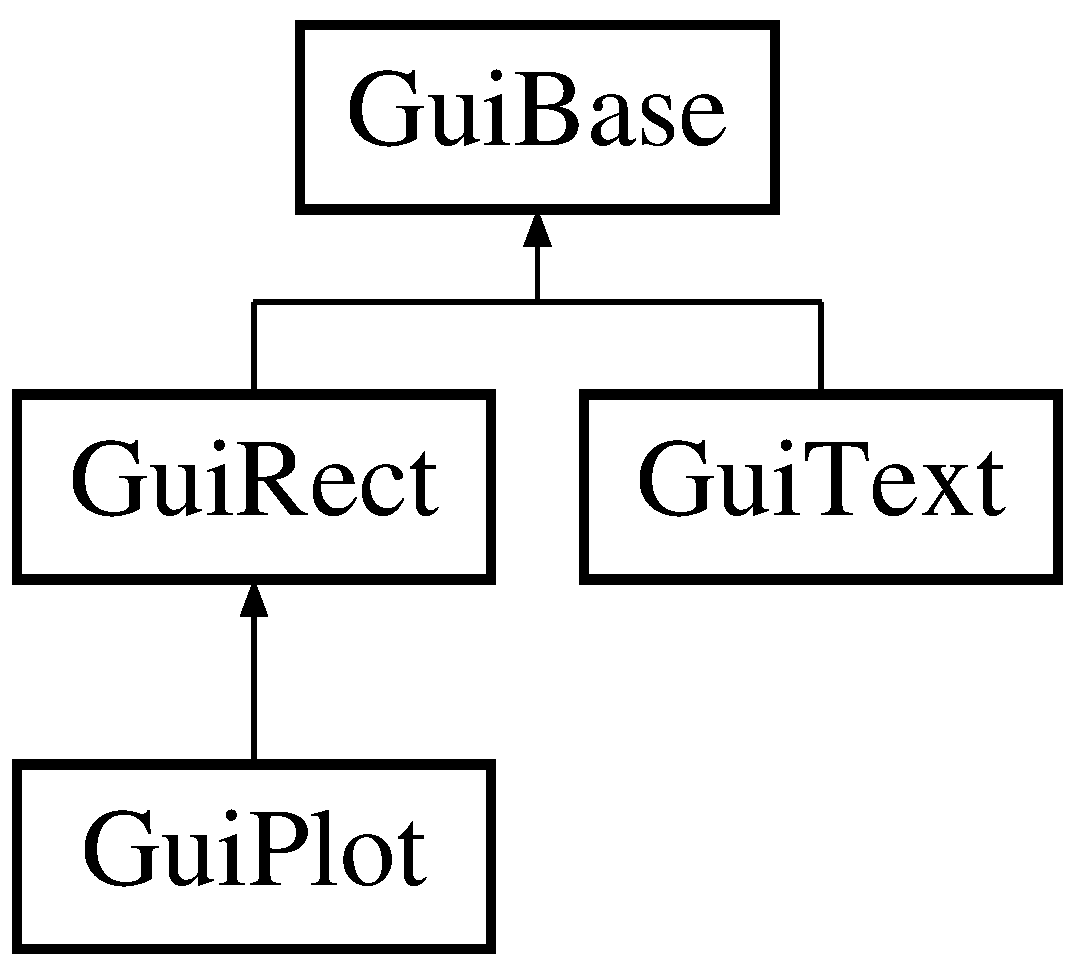
\includegraphics[height=3.000000cm]{class_gui_base}
\end{center}
\end{figure}
\subsection*{Public Types}
\begin{DoxyCompactItemize}
\item 
\hypertarget{class_gui_base_a0f3e57c1a942210072030196844b22eb}{typedef std\-::deque$<$ \hyperlink{class_gui_base}{Gui\-Base} $\ast$ $>$ \hyperlink{class_gui_base_a0f3e57c1a942210072030196844b22eb}{Gui\-Base\-Deque}}\label{class_gui_base_a0f3e57c1a942210072030196844b22eb}

\begin{DoxyCompactList}\small\item\em A deque of Gui\-Base$\ast$ nodes. \end{DoxyCompactList}\item 
\hypertarget{class_gui_base_a38bc5568225f8923caf32f75716cc354}{typedef Gui\-Base\-Deque\-::iterator \hyperlink{class_gui_base_a38bc5568225f8923caf32f75716cc354}{Gui\-Base\-Deque\-Iter}}\label{class_gui_base_a38bc5568225f8923caf32f75716cc354}

\begin{DoxyCompactList}\small\item\em An iterator type for a deque of Gui\-Base$\ast$ nodes. \end{DoxyCompactList}\item 
\hypertarget{class_gui_base_ae7e0e9c9c8fe03ac1760b8bb74c46786}{typedef \\*
Gui\-Base\-Deque\-::reverse\-\_\-iterator \hyperlink{class_gui_base_ae7e0e9c9c8fe03ac1760b8bb74c46786}{Gui\-Base\-Deque\-Riter}}\label{class_gui_base_ae7e0e9c9c8fe03ac1760b8bb74c46786}

\begin{DoxyCompactList}\small\item\em A reverse iterator type for a deque of Gui\-Base$\ast$ nodes. \end{DoxyCompactList}\item 
\hypertarget{class_gui_base_a40106bc7f71c718672756d0668aa83eb}{typedef \\*
Gui\-Base\-Deque\-::const\-\_\-iterator \hyperlink{class_gui_base_a40106bc7f71c718672756d0668aa83eb}{Gui\-Base\-Deque\-Citer}}\label{class_gui_base_a40106bc7f71c718672756d0668aa83eb}

\begin{DoxyCompactList}\small\item\em A const iterator type for a deque of Gui\-Base$\ast$ nodes. \end{DoxyCompactList}\end{DoxyCompactItemize}
\subsection*{Public Member Functions}
\begin{DoxyCompactItemize}
\item 
\hypertarget{class_gui_base_a9709f9e456c49c05094e7d2f96fef5f0}{\hyperlink{class_gui_base_a9709f9e456c49c05094e7d2f96fef5f0}{Gui\-Base} ()}\label{class_gui_base_a9709f9e456c49c05094e7d2f96fef5f0}

\begin{DoxyCompactList}\small\item\em Basic constructor. \end{DoxyCompactList}\item 
\hypertarget{class_gui_base_a6ced3adb2ad93c9970ef415eaa5ffecb}{virtual \hyperlink{class_gui_base_a6ced3adb2ad93c9970ef415eaa5ffecb}{$\sim$\-Gui\-Base} ()}\label{class_gui_base_a6ced3adb2ad93c9970ef415eaa5ffecb}

\begin{DoxyCompactList}\small\item\em Virtual destructor. \end{DoxyCompactList}\item 
\hypertarget{class_gui_base_af8f620fb195f78481f1487f98f09373e}{void \hyperlink{class_gui_base_af8f620fb195f78481f1487f98f09373e}{set\-Name} (const std\-::string \&i\-Name)}\label{class_gui_base_af8f620fb195f78481f1487f98f09373e}

\begin{DoxyCompactList}\small\item\em Sets the node's name label. \end{DoxyCompactList}\item 
\hypertarget{class_gui_base_a3108caaa4336deed6a28134d59a5b69b}{const std\-::string \& \hyperlink{class_gui_base_a3108caaa4336deed6a28134d59a5b69b}{get\-Name} ()}\label{class_gui_base_a3108caaa4336deed6a28134d59a5b69b}

\begin{DoxyCompactList}\small\item\em Returns the node's name label. \end{DoxyCompactList}\item 
\hypertarget{class_gui_base_a202171c06ea2331c8d97cb168b950eba}{void \hyperlink{class_gui_base_a202171c06ea2331c8d97cb168b950eba}{set\-Visibility} (const bool \&i\-Visible)}\label{class_gui_base_a202171c06ea2331c8d97cb168b950eba}

\begin{DoxyCompactList}\small\item\em Sets the node's visibility status. \end{DoxyCompactList}\item 
\hypertarget{class_gui_base_a80bfb0340d9997bed8602bbdf68d1c3a}{bool \hyperlink{class_gui_base_a80bfb0340d9997bed8602bbdf68d1c3a}{get\-Visibility} () const }\label{class_gui_base_a80bfb0340d9997bed8602bbdf68d1c3a}

\begin{DoxyCompactList}\small\item\em Returns the node's visibility status. \end{DoxyCompactList}\item 
\hypertarget{class_gui_base_a4f9320c8800cf8ee4286cf285b94354d}{void \hyperlink{class_gui_base_a4f9320c8800cf8ee4286cf285b94354d}{deep\-Draw} ()}\label{class_gui_base_a4f9320c8800cf8ee4286cf285b94354d}

\begin{DoxyCompactList}\small\item\em The node's deep draw handler. \end{DoxyCompactList}\item 
\hypertarget{class_gui_base_abad037dd46417bb2170d0981751da6e9}{virtual void \hyperlink{class_gui_base_abad037dd46417bb2170d0981751da6e9}{draw} ()}\label{class_gui_base_abad037dd46417bb2170d0981751da6e9}

\begin{DoxyCompactList}\small\item\em An overloadable draw method. \end{DoxyCompactList}\item 
\hypertarget{class_gui_base_a82f0c6988d8462ebe533ad8fed99cd78}{bool \hyperlink{class_gui_base_a82f0c6988d8462ebe533ad8fed99cd78}{deep\-Mouse\-Move} (ci\-::app\-::\-Mouse\-Event i\-Event)}\label{class_gui_base_a82f0c6988d8462ebe533ad8fed99cd78}

\begin{DoxyCompactList}\small\item\em The node's deep event-\/handler for mouse\-Move events. \end{DoxyCompactList}\item 
\hypertarget{class_gui_base_af5cfa808f38454d6b33d90a72ca13f52}{bool \hyperlink{class_gui_base_af5cfa808f38454d6b33d90a72ca13f52}{deep\-Mouse\-Down} (ci\-::app\-::\-Mouse\-Event i\-Event)}\label{class_gui_base_af5cfa808f38454d6b33d90a72ca13f52}

\begin{DoxyCompactList}\small\item\em The node's deep event-\/handler for mouse\-Down events. \end{DoxyCompactList}\item 
\hypertarget{class_gui_base_a9c08b19d2015b258344e5beb250166b9}{bool \hyperlink{class_gui_base_a9c08b19d2015b258344e5beb250166b9}{deep\-Mouse\-Drag} (ci\-::app\-::\-Mouse\-Event i\-Event)}\label{class_gui_base_a9c08b19d2015b258344e5beb250166b9}

\begin{DoxyCompactList}\small\item\em The node's deep event-\/handler for mouse\-Drag events. \end{DoxyCompactList}\item 
\hypertarget{class_gui_base_a5c32547724d1bb464a5de324be6d952e}{bool \hyperlink{class_gui_base_a5c32547724d1bb464a5de324be6d952e}{deep\-Mouse\-Up} (ci\-::app\-::\-Mouse\-Event i\-Event)}\label{class_gui_base_a5c32547724d1bb464a5de324be6d952e}

\begin{DoxyCompactList}\small\item\em The node's deep event-\/handler for mouse\-Up events. \end{DoxyCompactList}\item 
\hypertarget{class_gui_base_aa7dc9f856dcdad3957fccdb3ffed73a1}{virtual bool \hyperlink{class_gui_base_aa7dc9f856dcdad3957fccdb3ffed73a1}{mouse\-Move} (ci\-::app\-::\-Mouse\-Event i\-Event)}\label{class_gui_base_aa7dc9f856dcdad3957fccdb3ffed73a1}

\begin{DoxyCompactList}\small\item\em An overloadable event-\/handler for mouse\-Move events. \end{DoxyCompactList}\item 
\hypertarget{class_gui_base_ab8dad5df129e93169feef4a5ff6fa01c}{virtual bool \hyperlink{class_gui_base_ab8dad5df129e93169feef4a5ff6fa01c}{mouse\-Down} (ci\-::app\-::\-Mouse\-Event i\-Event)}\label{class_gui_base_ab8dad5df129e93169feef4a5ff6fa01c}

\begin{DoxyCompactList}\small\item\em An overloadable event-\/handler for mouse\-Down events. \end{DoxyCompactList}\item 
\hypertarget{class_gui_base_aabaebece81c1da9dd999facbaf4069f7}{virtual bool \hyperlink{class_gui_base_aabaebece81c1da9dd999facbaf4069f7}{mouse\-Drag} (ci\-::app\-::\-Mouse\-Event i\-Event)}\label{class_gui_base_aabaebece81c1da9dd999facbaf4069f7}

\begin{DoxyCompactList}\small\item\em An overloadable event-\/handler for mouse\-Drag events. \end{DoxyCompactList}\item 
\hypertarget{class_gui_base_a4b117a85faac9c1ad05232cc26cc72b2}{virtual bool \hyperlink{class_gui_base_a4b117a85faac9c1ad05232cc26cc72b2}{mouse\-Up} (ci\-::app\-::\-Mouse\-Event i\-Event)}\label{class_gui_base_a4b117a85faac9c1ad05232cc26cc72b2}

\begin{DoxyCompactList}\small\item\em An overloadable event-\/handler for mouse\-Up events. \end{DoxyCompactList}\item 
\hypertarget{class_gui_base_a5b208c23add4471fe5a84ad9b72dec88}{bool \hyperlink{class_gui_base_a5b208c23add4471fe5a84ad9b72dec88}{deep\-Key\-Down} (ci\-::app\-::\-Key\-Event i\-Event)}\label{class_gui_base_a5b208c23add4471fe5a84ad9b72dec88}

\begin{DoxyCompactList}\small\item\em The node's deep event-\/handler for key\-Down events. \end{DoxyCompactList}\item 
\hypertarget{class_gui_base_a3497b3630f38a9235038e725a0ed516d}{bool \hyperlink{class_gui_base_a3497b3630f38a9235038e725a0ed516d}{deep\-Key\-Up} (ci\-::app\-::\-Key\-Event i\-Event)}\label{class_gui_base_a3497b3630f38a9235038e725a0ed516d}

\begin{DoxyCompactList}\small\item\em The node's deep event-\/handler for key\-Up events. \end{DoxyCompactList}\item 
\hypertarget{class_gui_base_aff89c3ffda887abb5ccce31ba5c07425}{virtual bool \hyperlink{class_gui_base_aff89c3ffda887abb5ccce31ba5c07425}{key\-Down} (ci\-::app\-::\-Key\-Event i\-Event)}\label{class_gui_base_aff89c3ffda887abb5ccce31ba5c07425}

\begin{DoxyCompactList}\small\item\em An overloadable event-\/handler for key\-Down events. \end{DoxyCompactList}\item 
\hypertarget{class_gui_base_a5ef639091768571edc0c08a1c8544ded}{virtual bool \hyperlink{class_gui_base_a5ef639091768571edc0c08a1c8544ded}{key\-Up} (ci\-::app\-::\-Key\-Event i\-Event)}\label{class_gui_base_a5ef639091768571edc0c08a1c8544ded}

\begin{DoxyCompactList}\small\item\em An overloadable event-\/handler for key\-Up events. \end{DoxyCompactList}\item 
\hypertarget{class_gui_base_aaf56570a4104f842b8b1fb533342b198}{bool \hyperlink{class_gui_base_aaf56570a4104f842b8b1fb533342b198}{has\-Parent} () const }\label{class_gui_base_aaf56570a4104f842b8b1fb533342b198}

\begin{DoxyCompactList}\small\item\em Returns true if the node has a parent node. \end{DoxyCompactList}\item 
\hypertarget{class_gui_base_a92e8c890aca536b6c542dae8b16a2b36}{\hyperlink{class_gui_base}{Gui\-Base} $\ast$ \hyperlink{class_gui_base_a92e8c890aca536b6c542dae8b16a2b36}{get\-Parent} () const }\label{class_gui_base_a92e8c890aca536b6c542dae8b16a2b36}

\begin{DoxyCompactList}\small\item\em Returns the node's parent if one exists, otherwise N\-U\-L\-L. \end{DoxyCompactList}\item 
\hypertarget{class_gui_base_a306709c52a6e4fb06ae58f4a9061d2e9}{void \hyperlink{class_gui_base_a306709c52a6e4fb06ae58f4a9061d2e9}{set\-Parent} (\hyperlink{class_gui_base}{Gui\-Base} $\ast$i\-Parent)}\label{class_gui_base_a306709c52a6e4fb06ae58f4a9061d2e9}

\begin{DoxyCompactList}\small\item\em Sets the node's parent. \end{DoxyCompactList}\item 
\hypertarget{class_gui_base_a774b4aac5d662980acca69de5c9ac024}{bool \hyperlink{class_gui_base_a774b4aac5d662980acca69de5c9ac024}{has\-Children} () const }\label{class_gui_base_a774b4aac5d662980acca69de5c9ac024}

\begin{DoxyCompactList}\small\item\em Returns true if the node has children nodes. \end{DoxyCompactList}\item 
\hypertarget{class_gui_base_a3b03dd2b4bc97f86d73b183e6367caf1}{\hyperlink{class_gui_base_a0f3e57c1a942210072030196844b22eb}{Gui\-Base\-Deque} \& \hyperlink{class_gui_base_a3b03dd2b4bc97f86d73b183e6367caf1}{get\-Children} ()}\label{class_gui_base_a3b03dd2b4bc97f86d73b183e6367caf1}

\begin{DoxyCompactList}\small\item\em Returns a reference to the child node deque. \end{DoxyCompactList}\item 
\hypertarget{class_gui_base_a2ed7f1bcbc74e60224d563b26231c7ed}{const \hyperlink{class_gui_base_a0f3e57c1a942210072030196844b22eb}{Gui\-Base\-Deque} \& \hyperlink{class_gui_base_a2ed7f1bcbc74e60224d563b26231c7ed}{get\-Children} () const }\label{class_gui_base_a2ed7f1bcbc74e60224d563b26231c7ed}

\begin{DoxyCompactList}\small\item\em Returns a const reference to the child node deque. \end{DoxyCompactList}\item 
\hypertarget{class_gui_base_af9a34d3430994bf192ac23848c98dac4}{void \hyperlink{class_gui_base_af9a34d3430994bf192ac23848c98dac4}{add\-Child} (\hyperlink{class_gui_base}{Gui\-Base} $\ast$i\-Child)}\label{class_gui_base_af9a34d3430994bf192ac23848c98dac4}

\begin{DoxyCompactList}\small\item\em Adds the given node as a child of this node. \end{DoxyCompactList}\item 
\hypertarget{class_gui_base_a84219d452d3239cd82d8032bbe04ef72}{void \hyperlink{class_gui_base_a84219d452d3239cd82d8032bbe04ef72}{set\-Position} (const ci\-::\-Vec2f \&i\-Position)}\label{class_gui_base_a84219d452d3239cd82d8032bbe04ef72}

\begin{DoxyCompactList}\small\item\em Sets the node's fixed position. \end{DoxyCompactList}\item 
\hypertarget{class_gui_base_a1426d946b2d63f4c0b66e49daabf8b40}{void \hyperlink{class_gui_base_a1426d946b2d63f4c0b66e49daabf8b40}{set\-Position} (const float \&i\-Position\-X, const float \&i\-Position\-Y)}\label{class_gui_base_a1426d946b2d63f4c0b66e49daabf8b40}

\begin{DoxyCompactList}\small\item\em Sets the node's fixed position. \end{DoxyCompactList}\item 
\hypertarget{class_gui_base_a48e9f988d580de29790cc92032c1bdfd}{void \hyperlink{class_gui_base_a48e9f988d580de29790cc92032c1bdfd}{set\-Position\-X} (const float \&i\-Position\-X)}\label{class_gui_base_a48e9f988d580de29790cc92032c1bdfd}

\begin{DoxyCompactList}\small\item\em Sets the node's fixed x-\/position. \end{DoxyCompactList}\item 
\hypertarget{class_gui_base_adf16803de83c7ddd40262ae8185ce818}{void \hyperlink{class_gui_base_adf16803de83c7ddd40262ae8185ce818}{set\-Position\-Y} (const float \&i\-Position\-Y)}\label{class_gui_base_adf16803de83c7ddd40262ae8185ce818}

\begin{DoxyCompactList}\small\item\em Sets the node's fixed y-\/position. \end{DoxyCompactList}\item 
\hypertarget{class_gui_base_af86716fca942b5b0624018365a0f23c1}{void \hyperlink{class_gui_base_af86716fca942b5b0624018365a0f23c1}{set\-Relative\-Position} (const ci\-::\-Vec2f \&i\-Position)}\label{class_gui_base_af86716fca942b5b0624018365a0f23c1}

\begin{DoxyCompactList}\small\item\em Sets the node's relative position. \end{DoxyCompactList}\item 
\hypertarget{class_gui_base_a1ed4c24befd781d83997c2484a595560}{void \hyperlink{class_gui_base_a1ed4c24befd781d83997c2484a595560}{set\-Relative\-Position} (const float \&i\-Position\-X, const float \&i\-Position\-Y)}\label{class_gui_base_a1ed4c24befd781d83997c2484a595560}

\begin{DoxyCompactList}\small\item\em Sets the node's relative position. \end{DoxyCompactList}\item 
\hypertarget{class_gui_base_a7531a4234bff4e52b5305a6f679fa424}{void \hyperlink{class_gui_base_a7531a4234bff4e52b5305a6f679fa424}{set\-Relative\-Position\-X} (const float \&i\-Position\-X)}\label{class_gui_base_a7531a4234bff4e52b5305a6f679fa424}

\begin{DoxyCompactList}\small\item\em Sets the node's relative x-\/position. \end{DoxyCompactList}\item 
\hypertarget{class_gui_base_a1a5f52bc55ced711f170369ec7b5e9f6}{void \hyperlink{class_gui_base_a1a5f52bc55ced711f170369ec7b5e9f6}{set\-Relative\-Position\-Y} (const float \&i\-Position\-Y)}\label{class_gui_base_a1a5f52bc55ced711f170369ec7b5e9f6}

\begin{DoxyCompactList}\small\item\em Sets the node's relative y-\/position. \end{DoxyCompactList}\item 
\hypertarget{class_gui_base_a4635594f079588835e5883fc6fecaee6}{ci\-::\-Vec2f \hyperlink{class_gui_base_a4635594f079588835e5883fc6fecaee6}{get\-Position} () const }\label{class_gui_base_a4635594f079588835e5883fc6fecaee6}

\begin{DoxyCompactList}\small\item\em Returns the node's screen position. \end{DoxyCompactList}\item 
\hypertarget{class_gui_base_a6246f3646b4ea1b4a441b3ab03236ed0}{ci\-::\-Vec2f \hyperlink{class_gui_base_a6246f3646b4ea1b4a441b3ab03236ed0}{get\-Local\-Position} () const }\label{class_gui_base_a6246f3646b4ea1b4a441b3ab03236ed0}

\begin{DoxyCompactList}\small\item\em Returns the node's local position within its parent. \end{DoxyCompactList}\item 
\hypertarget{class_gui_base_a98fed57a0ec8a7e802c30c69f5f05e92}{void \hyperlink{class_gui_base_a98fed57a0ec8a7e802c30c69f5f05e92}{set\-Dimension} (const ci\-::\-Vec2f \&i\-Dimension)}\label{class_gui_base_a98fed57a0ec8a7e802c30c69f5f05e92}

\begin{DoxyCompactList}\small\item\em Sets the node's fixed dimension. \end{DoxyCompactList}\item 
\hypertarget{class_gui_base_a52e34244954a8d3fd17d5a40809d6491}{void \hyperlink{class_gui_base_a52e34244954a8d3fd17d5a40809d6491}{set\-Dimension} (const float \&i\-Dimension\-X, const float \&i\-Dimension\-Y)}\label{class_gui_base_a52e34244954a8d3fd17d5a40809d6491}

\begin{DoxyCompactList}\small\item\em Sets the node's fixed dimension. \end{DoxyCompactList}\item 
\hypertarget{class_gui_base_a63efdb39227f4803b29a9ed8d2d7595c}{void \hyperlink{class_gui_base_a63efdb39227f4803b29a9ed8d2d7595c}{set\-Dimension\-X} (const float \&i\-Dimension\-X)}\label{class_gui_base_a63efdb39227f4803b29a9ed8d2d7595c}

\begin{DoxyCompactList}\small\item\em Sets the node's fixed x-\/dimension. \end{DoxyCompactList}\item 
\hypertarget{class_gui_base_a465d2dac52ef361d32fc0da11fc96037}{void \hyperlink{class_gui_base_a465d2dac52ef361d32fc0da11fc96037}{set\-Dimension\-Y} (const float \&i\-Dimension\-Y)}\label{class_gui_base_a465d2dac52ef361d32fc0da11fc96037}

\begin{DoxyCompactList}\small\item\em Sets the node's fixed y-\/dimension. \end{DoxyCompactList}\item 
\hypertarget{class_gui_base_aec9af0c20f3450a724b7b2351285bb18}{void \hyperlink{class_gui_base_aec9af0c20f3450a724b7b2351285bb18}{set\-Relative\-Dimension} (const ci\-::\-Vec2f \&i\-Dimension)}\label{class_gui_base_aec9af0c20f3450a724b7b2351285bb18}

\begin{DoxyCompactList}\small\item\em Sets the node's relative dimension. \end{DoxyCompactList}\item 
\hypertarget{class_gui_base_a449cadd489954fcf58a3563b410f3c60}{void \hyperlink{class_gui_base_a449cadd489954fcf58a3563b410f3c60}{set\-Relative\-Dimension} (const float \&i\-Dimension\-X, const float \&i\-Dimension\-Y)}\label{class_gui_base_a449cadd489954fcf58a3563b410f3c60}

\begin{DoxyCompactList}\small\item\em Sets the node's relative dimension. \end{DoxyCompactList}\item 
\hypertarget{class_gui_base_a7813f46fcb0b4072484ecd71f41998de}{void \hyperlink{class_gui_base_a7813f46fcb0b4072484ecd71f41998de}{set\-Relative\-Dimension\-X} (const float \&i\-Dimension\-X)}\label{class_gui_base_a7813f46fcb0b4072484ecd71f41998de}

\begin{DoxyCompactList}\small\item\em Sets the node's relative x-\/dimension. \end{DoxyCompactList}\item 
\hypertarget{class_gui_base_a52fe756effdc1e619fad534b67f168ec}{void \hyperlink{class_gui_base_a52fe756effdc1e619fad534b67f168ec}{set\-Relative\-Dimension\-Y} (const float \&i\-Dimension\-Y)}\label{class_gui_base_a52fe756effdc1e619fad534b67f168ec}

\begin{DoxyCompactList}\small\item\em Sets the node's relative y-\/dimension. \end{DoxyCompactList}\item 
\hypertarget{class_gui_base_a940460c55f91a4132f871673f808e7a7}{ci\-::\-Vec2f \hyperlink{class_gui_base_a940460c55f91a4132f871673f808e7a7}{get\-Dimension} () const }\label{class_gui_base_a940460c55f91a4132f871673f808e7a7}

\begin{DoxyCompactList}\small\item\em Returns the node's screen dimension. \end{DoxyCompactList}\item 
\hypertarget{class_gui_base_a7a54ae06139a02532c51b1e198c24133}{float \hyperlink{class_gui_base_a7a54ae06139a02532c51b1e198c24133}{get\-Dimension\-X} () const }\label{class_gui_base_a7a54ae06139a02532c51b1e198c24133}

\begin{DoxyCompactList}\small\item\em Returns the node's screen x-\/dimension. \end{DoxyCompactList}\item 
\hypertarget{class_gui_base_af79e3089b3a018012e9acbd7fd29708a}{float \hyperlink{class_gui_base_af79e3089b3a018012e9acbd7fd29708a}{get\-Dimension\-Y} () const }\label{class_gui_base_af79e3089b3a018012e9acbd7fd29708a}

\begin{DoxyCompactList}\small\item\em Returns the node's screen y-\/dimension. \end{DoxyCompactList}\end{DoxyCompactItemize}
\subsection*{Protected Attributes}
\begin{DoxyCompactItemize}
\item 
\hypertarget{class_gui_base_ab0e76796e0274a3b538e44cda82a6f5f}{std\-::string \hyperlink{class_gui_base_ab0e76796e0274a3b538e44cda82a6f5f}{m\-Name}}\label{class_gui_base_ab0e76796e0274a3b538e44cda82a6f5f}

\begin{DoxyCompactList}\small\item\em The node's name. \end{DoxyCompactList}\item 
\hypertarget{class_gui_base_a07fc7363624a8d4c586775e7d68114cd}{bool \hyperlink{class_gui_base_a07fc7363624a8d4c586775e7d68114cd}{m\-Visible}}\label{class_gui_base_a07fc7363624a8d4c586775e7d68114cd}

\begin{DoxyCompactList}\small\item\em Flags whether the node is visible. \end{DoxyCompactList}\item 
\hypertarget{class_gui_base_a22d9fe30a7103f02e24396f8473e7317}{ci\-::\-Vec2f \hyperlink{class_gui_base_a22d9fe30a7103f02e24396f8473e7317}{m\-Position}}\label{class_gui_base_a22d9fe30a7103f02e24396f8473e7317}

\begin{DoxyCompactList}\small\item\em The node's position (either absolute or relative) \end{DoxyCompactList}\item 
\hypertarget{class_gui_base_a3f63f449843068c1472454de3fdf1462}{ci\-::\-Vec2f \hyperlink{class_gui_base_a3f63f449843068c1472454de3fdf1462}{m\-Dimension}}\label{class_gui_base_a3f63f449843068c1472454de3fdf1462}

\begin{DoxyCompactList}\small\item\em The node's dimension (either absolute or relative) \end{DoxyCompactList}\item 
\hypertarget{class_gui_base_af3c85abbf0a6aa3e27b679686837dc40}{Gui\-Flow \hyperlink{class_gui_base_af3c85abbf0a6aa3e27b679686837dc40}{m\-Flow\-X}}\label{class_gui_base_af3c85abbf0a6aa3e27b679686837dc40}

\begin{DoxyCompactList}\small\item\em The node's flow type for its x-\/position parameter. \end{DoxyCompactList}\item 
\hypertarget{class_gui_base_a22b6d4da341853066112fd67983a7f29}{Gui\-Flow \hyperlink{class_gui_base_a22b6d4da341853066112fd67983a7f29}{m\-Flow\-Y}}\label{class_gui_base_a22b6d4da341853066112fd67983a7f29}

\begin{DoxyCompactList}\small\item\em The node's flow type for its y-\/position parameter. \end{DoxyCompactList}\item 
\hypertarget{class_gui_base_a711b5c3c6b09852ac826186c922467a9}{Gui\-Flow \hyperlink{class_gui_base_a711b5c3c6b09852ac826186c922467a9}{m\-Flow\-W}}\label{class_gui_base_a711b5c3c6b09852ac826186c922467a9}

\begin{DoxyCompactList}\small\item\em The node's flow type for its width parameter. \end{DoxyCompactList}\item 
\hypertarget{class_gui_base_a2e9922cfe6e65ade8010d65afaa643a7}{Gui\-Flow \hyperlink{class_gui_base_a2e9922cfe6e65ade8010d65afaa643a7}{m\-Flow\-H}}\label{class_gui_base_a2e9922cfe6e65ade8010d65afaa643a7}

\begin{DoxyCompactList}\small\item\em The node's flow type for its height parameter. \end{DoxyCompactList}\item 
\hypertarget{class_gui_base_adc9738a64a6a41862ff8eb94d482b7c6}{\hyperlink{class_gui_base}{Gui\-Base} $\ast$ \hyperlink{class_gui_base_adc9738a64a6a41862ff8eb94d482b7c6}{m\-Parent}}\label{class_gui_base_adc9738a64a6a41862ff8eb94d482b7c6}

\begin{DoxyCompactList}\small\item\em A pointer to the node's parent. \end{DoxyCompactList}\item 
\hypertarget{class_gui_base_afce12e9e9fd92ce71e945cff1dc87b0e}{\hyperlink{class_gui_base_a0f3e57c1a942210072030196844b22eb}{Gui\-Base\-Deque} \hyperlink{class_gui_base_afce12e9e9fd92ce71e945cff1dc87b0e}{m\-Children}}\label{class_gui_base_afce12e9e9fd92ce71e945cff1dc87b0e}

\begin{DoxyCompactList}\small\item\em A deque of the node's children. \end{DoxyCompactList}\end{DoxyCompactItemize}


\subsection{Detailed Description}
A basic two-\/dimensional scenegraph node. 

The documentation for this class was generated from the following files\-:\begin{DoxyCompactItemize}
\item 
/\-Users/pjh/\-Desktop/\-Work/\-Teaching/\-Creative\-Evolution\-Course/core/include/gui/Gui\-Base.\-h\item 
/\-Users/pjh/\-Desktop/\-Work/\-Teaching/\-Creative\-Evolution\-Course/core/src/gui/Gui\-Base.\-cpp\end{DoxyCompactItemize}

\hypertarget{class_gui_plot}{\section{Gui\-Plot Class Reference}
\label{class_gui_plot}\index{Gui\-Plot@{Gui\-Plot}}
}


A 2\-D plotting widget.  




{\ttfamily \#include $<$Gui\-Plot.\-h$>$}

Inheritance diagram for Gui\-Plot\-:\begin{figure}[H]
\begin{center}
\leavevmode
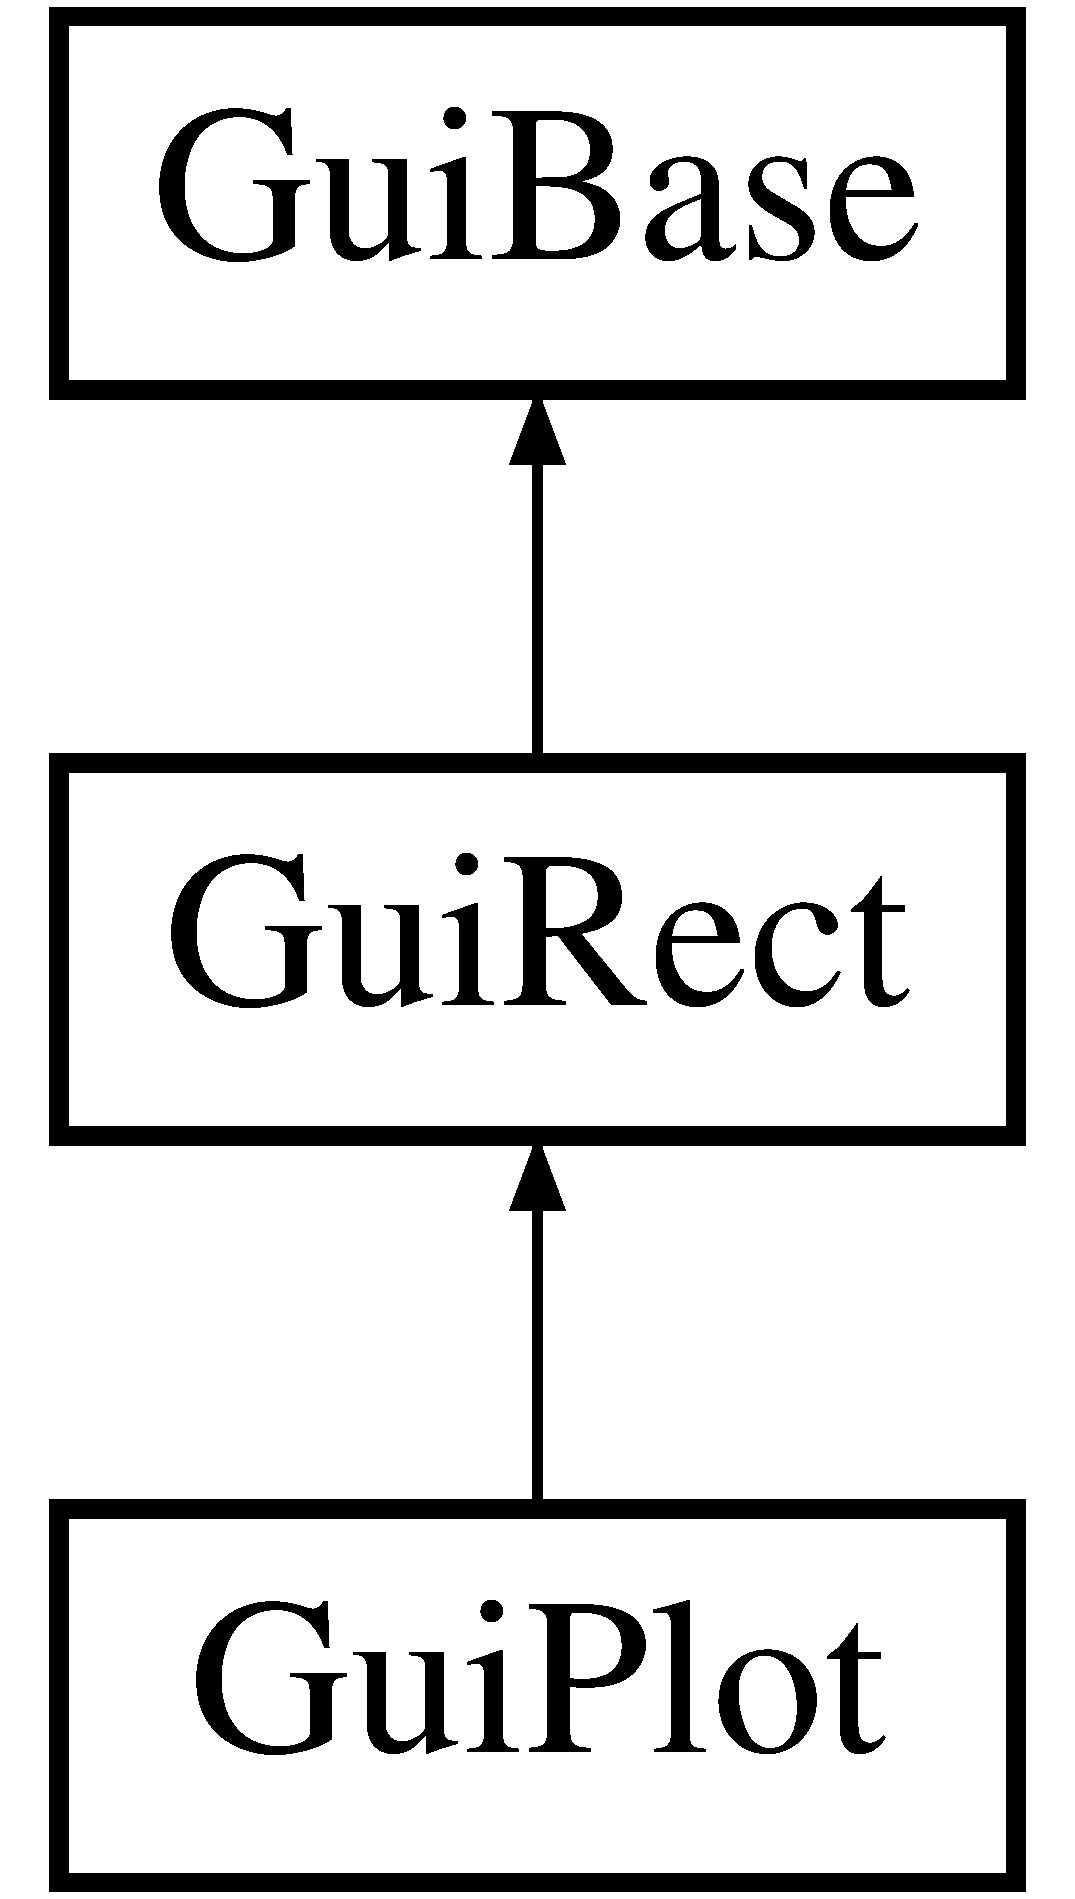
\includegraphics[height=3.000000cm]{class_gui_plot}
\end{center}
\end{figure}
\subsection*{Public Member Functions}
\begin{DoxyCompactItemize}
\item 
\hypertarget{class_gui_plot_a2498a68711d55cf7f368751f4607d64b}{\hyperlink{class_gui_plot_a2498a68711d55cf7f368751f4607d64b}{Gui\-Plot} (const std\-::string \&i\-Font\-Family\-Name=\char`\"{}\char`\"{}, \hyperlink{class_font_suitcase}{Font\-Suitcase} $\ast$i\-Font\-Suitcase\-Ref=N\-U\-L\-L)}\label{class_gui_plot_a2498a68711d55cf7f368751f4607d64b}

\begin{DoxyCompactList}\small\item\em Basic constructor. \end{DoxyCompactList}\item 
\hypertarget{class_gui_plot_ab27d0193bfdc446bb0602ed5643b4559}{virtual \hyperlink{class_gui_plot_ab27d0193bfdc446bb0602ed5643b4559}{$\sim$\-Gui\-Plot} ()}\label{class_gui_plot_ab27d0193bfdc446bb0602ed5643b4559}

\begin{DoxyCompactList}\small\item\em Virtual destructor. \end{DoxyCompactList}\item 
\hypertarget{class_gui_plot_a9934bd4298d6b193ceb383e885e799b0}{virtual void \hyperlink{class_gui_plot_a9934bd4298d6b193ceb383e885e799b0}{draw} ()}\label{class_gui_plot_a9934bd4298d6b193ceb383e885e799b0}

\begin{DoxyCompactList}\small\item\em An overloadable draw method. \end{DoxyCompactList}\item 
\hypertarget{class_gui_plot_a1ada61adcf5a6822789d64d498d4db53}{virtual bool \hyperlink{class_gui_plot_a1ada61adcf5a6822789d64d498d4db53}{mouse\-Move} (ci\-::app\-::\-Mouse\-Event i\-Event)}\label{class_gui_plot_a1ada61adcf5a6822789d64d498d4db53}

\begin{DoxyCompactList}\small\item\em Overloadable mouse move event callback method. \end{DoxyCompactList}\item 
\hypertarget{class_gui_plot_a662400c9664d5db58a9a0fff20a86724}{virtual bool \hyperlink{class_gui_plot_a662400c9664d5db58a9a0fff20a86724}{mouse\-Down} (ci\-::app\-::\-Mouse\-Event i\-Event)}\label{class_gui_plot_a662400c9664d5db58a9a0fff20a86724}

\begin{DoxyCompactList}\small\item\em Overloadable mouse down event callback method. \end{DoxyCompactList}\item 
\hypertarget{class_gui_plot_a20d1f7a342435f84ece58f982b93ab73}{virtual bool \hyperlink{class_gui_plot_a20d1f7a342435f84ece58f982b93ab73}{mouse\-Drag} (ci\-::app\-::\-Mouse\-Event i\-Event)}\label{class_gui_plot_a20d1f7a342435f84ece58f982b93ab73}

\begin{DoxyCompactList}\small\item\em Overloadable mouse drag event callback method. \end{DoxyCompactList}\item 
\hypertarget{class_gui_plot_a8f6863d909939793411aa4851bd352b2}{virtual bool \hyperlink{class_gui_plot_a8f6863d909939793411aa4851bd352b2}{mouse\-Up} (ci\-::app\-::\-Mouse\-Event i\-Event)}\label{class_gui_plot_a8f6863d909939793411aa4851bd352b2}

\begin{DoxyCompactList}\small\item\em Overloadable mouse up event callback method. \end{DoxyCompactList}\item 
\hypertarget{class_gui_plot_a3df99256140c63ae43b9ba8faf0d4510}{void \hyperlink{class_gui_plot_a3df99256140c63ae43b9ba8faf0d4510}{clear\-Inputs} ()}\label{class_gui_plot_a3df99256140c63ae43b9ba8faf0d4510}

\begin{DoxyCompactList}\small\item\em Removes all data inputs from the plotter. \end{DoxyCompactList}\item 
\hypertarget{class_gui_plot_a290cf385f061efe1fedec0064f1a00ea}{void \hyperlink{class_gui_plot_a290cf385f061efe1fedec0064f1a00ea}{add\-Input} (const ci\-::\-Poly\-Line2f \&i\-Input, const ci\-::\-Color\-A \&i\-Color)}\label{class_gui_plot_a290cf385f061efe1fedec0064f1a00ea}

\begin{DoxyCompactList}\small\item\em Adds a ci\-::\-Poly\-Line2f data input to the plotter. \end{DoxyCompactList}\item 
\hypertarget{class_gui_plot_ad1ef90cad89b9ef731571f9b14df38c6}{void \hyperlink{class_gui_plot_ad1ef90cad89b9ef731571f9b14df38c6}{add\-Input} (Plotter\-Data\-Ref i\-Data\-Ref)}\label{class_gui_plot_ad1ef90cad89b9ef731571f9b14df38c6}

\begin{DoxyCompactList}\small\item\em Adds a Plotter\-Data\-Ref data input to the plotter. \end{DoxyCompactList}\item 
\hypertarget{class_gui_plot_a8394bf0d66cf21991d1e1aab7bb02ecc}{void \hyperlink{class_gui_plot_a8394bf0d66cf21991d1e1aab7bb02ecc}{remove\-Input} (Plotter\-Data\-Ref i\-Data\-Ref)}\label{class_gui_plot_a8394bf0d66cf21991d1e1aab7bb02ecc}

\begin{DoxyCompactList}\small\item\em Removes the given Plotter\-Data\-Ref data input from the plotter. \end{DoxyCompactList}\item 
\hypertarget{class_gui_plot_ae9cdb3ce87cd2e2a6fdf3de900ff0c7f}{void \hyperlink{class_gui_plot_ae9cdb3ce87cd2e2a6fdf3de900ff0c7f}{set\-X\-Range} (const float \&i\-Min, const float \&i\-Max)}\label{class_gui_plot_ae9cdb3ce87cd2e2a6fdf3de900ff0c7f}

\begin{DoxyCompactList}\small\item\em Sets the display range for the graph's x-\/axis. \end{DoxyCompactList}\item 
\hypertarget{class_gui_plot_a9242906c392d26d67b3c196a3b2321ea}{void \hyperlink{class_gui_plot_a9242906c392d26d67b3c196a3b2321ea}{set\-Y\-Range} (const float \&i\-Min, const float \&i\-Max)}\label{class_gui_plot_a9242906c392d26d67b3c196a3b2321ea}

\begin{DoxyCompactList}\small\item\em Sets the display range for the graph's y-\/axis. \end{DoxyCompactList}\item 
\hypertarget{class_gui_plot_a911632acbcb10fbbab823503a84898e9}{void \hyperlink{class_gui_plot_a911632acbcb10fbbab823503a84898e9}{set\-Origin\-Color} (const ci\-::\-Color\-A \&i\-Color)}\label{class_gui_plot_a911632acbcb10fbbab823503a84898e9}

\begin{DoxyCompactList}\small\item\em Sets the origin line color. \end{DoxyCompactList}\item 
\hypertarget{class_gui_plot_abaec0cb9deef925de4ea44f68a8cd5de}{const ci\-::\-Color\-A \& \hyperlink{class_gui_plot_abaec0cb9deef925de4ea44f68a8cd5de}{get\-Origin\-Color} () const }\label{class_gui_plot_abaec0cb9deef925de4ea44f68a8cd5de}

\begin{DoxyCompactList}\small\item\em Returns the origin line color. \end{DoxyCompactList}\item 
\hypertarget{class_gui_plot_a67df433b9f22adf9bdadecb6a5b685b0}{void \hyperlink{class_gui_plot_a67df433b9f22adf9bdadecb6a5b685b0}{set\-Origin\-Weight} (const float \&i\-Weight)}\label{class_gui_plot_a67df433b9f22adf9bdadecb6a5b685b0}

\begin{DoxyCompactList}\small\item\em Sets the origin line width. \end{DoxyCompactList}\item 
\hypertarget{class_gui_plot_aab5051cf6575fbe38bf9e326f9ce9780}{const float \& \hyperlink{class_gui_plot_aab5051cf6575fbe38bf9e326f9ce9780}{get\-Origin\-Weight} () const }\label{class_gui_plot_aab5051cf6575fbe38bf9e326f9ce9780}

\begin{DoxyCompactList}\small\item\em Returns the origin line width. \end{DoxyCompactList}\item 
\hypertarget{class_gui_plot_aa52f853cd41fd11e9c9927c7cff2c2ee}{void \hyperlink{class_gui_plot_aa52f853cd41fd11e9c9927c7cff2c2ee}{set\-Grid\-Color} (const ci\-::\-Color\-A \&i\-Color)}\label{class_gui_plot_aa52f853cd41fd11e9c9927c7cff2c2ee}

\begin{DoxyCompactList}\small\item\em Sets the grid line color. \end{DoxyCompactList}\item 
\hypertarget{class_gui_plot_a471ad0596b9f4e9bc57c68704343771f}{const ci\-::\-Color\-A \& \hyperlink{class_gui_plot_a471ad0596b9f4e9bc57c68704343771f}{get\-Grid\-Color} () const }\label{class_gui_plot_a471ad0596b9f4e9bc57c68704343771f}

\begin{DoxyCompactList}\small\item\em Returns the grid line color. \end{DoxyCompactList}\item 
\hypertarget{class_gui_plot_a6e7eb87c0794a5ab3b86aa8b316a0818}{void \hyperlink{class_gui_plot_a6e7eb87c0794a5ab3b86aa8b316a0818}{set\-Grid\-Weight} (const float \&i\-Weight)}\label{class_gui_plot_a6e7eb87c0794a5ab3b86aa8b316a0818}

\begin{DoxyCompactList}\small\item\em Sets the grid line width. \end{DoxyCompactList}\item 
\hypertarget{class_gui_plot_ae9cd92ed86587648db2148e69e93ed7e}{const float \& \hyperlink{class_gui_plot_ae9cd92ed86587648db2148e69e93ed7e}{get\-Grid\-Weight} () const }\label{class_gui_plot_ae9cd92ed86587648db2148e69e93ed7e}

\begin{DoxyCompactList}\small\item\em Returns the grid line width. \end{DoxyCompactList}\end{DoxyCompactItemize}
\subsection*{Protected Member Functions}
\begin{DoxyCompactItemize}
\item 
\hypertarget{class_gui_plot_a718bfecbf285f346fb31cae1ab2cb085}{virtual void \hyperlink{class_gui_plot_a718bfecbf285f346fb31cae1ab2cb085}{recompute\-Formatting} ()}\label{class_gui_plot_a718bfecbf285f346fb31cae1ab2cb085}

\begin{DoxyCompactList}\small\item\em An overloadable method that is evoked when the widget requires updating. \end{DoxyCompactList}\item 
\hypertarget{class_gui_plot_aeb458e8d702ec1eed13ddf3f4fe1f492}{void \hyperlink{class_gui_plot_aeb458e8d702ec1eed13ddf3f4fe1f492}{deep\-Recompute\-Formatting} ()}\label{class_gui_plot_aeb458e8d702ec1eed13ddf3f4fe1f492}

\begin{DoxyCompactList}\small\item\em A protected method that is evoked automatically when the widget requires updating. \end{DoxyCompactList}\item 
\hypertarget{class_gui_plot_a0f3e7eb075608be8efbdc7a667e48f26}{std\-::string \hyperlink{class_gui_plot_a0f3e7eb075608be8efbdc7a667e48f26}{get\-Vertex\-Label\-String} (const float \&i\-X, const float \&i\-Y)}\label{class_gui_plot_a0f3e7eb075608be8efbdc7a667e48f26}

\begin{DoxyCompactList}\small\item\em Returns a formatted string representing the input 2\-D coordinate. \end{DoxyCompactList}\item 
\hypertarget{class_gui_plot_a6efee73c07e1a6eab9e574e3f875d2ad}{bool \hyperlink{class_gui_plot_a6efee73c07e1a6eab9e574e3f875d2ad}{screen\-To\-Graph\-Coord} (const ci\-::\-Vec2f \&i\-Screen\-Coord, ci\-::\-Vec2f \&o\-Graph\-Coord, ci\-::\-Vec2f \&o\-Widget\-Relative\-Coord)}\label{class_gui_plot_a6efee73c07e1a6eab9e574e3f875d2ad}

\begin{DoxyCompactList}\small\item\em Returns true if given screen coordinate is within rect and if so, outputs adjusted graph and widget-\/relative coordinates as parameters. \end{DoxyCompactList}\item 
\hypertarget{class_gui_plot_af3bbbc33672c3aa8d33566b4e215fb52}{float \hyperlink{class_gui_plot_af3bbbc33672c3aa8d33566b4e215fb52}{round\-To\-Nearest} (const float \&i\-Value, const float \&i\-Interval)}\label{class_gui_plot_af3bbbc33672c3aa8d33566b4e215fb52}

\begin{DoxyCompactList}\small\item\em Returns the input value rounded to the nearest interval. \end{DoxyCompactList}\end{DoxyCompactItemize}
\subsection*{Protected Attributes}
\begin{DoxyCompactItemize}
\item 
\hypertarget{class_gui_plot_aa53372b5d96d2a55ebd85d0e02b49da4}{Plotter\-Data\-Ref\-Vec \hyperlink{class_gui_plot_aa53372b5d96d2a55ebd85d0e02b49da4}{m\-Inputs}}\label{class_gui_plot_aa53372b5d96d2a55ebd85d0e02b49da4}

\begin{DoxyCompactList}\small\item\em A vector of input references to be plotted. \end{DoxyCompactList}\item 
\hypertarget{class_gui_plot_a340e4fa2f245e2cb134102d5f1b9e0b4}{ci\-::\-Rectf \hyperlink{class_gui_plot_a340e4fa2f245e2cb134102d5f1b9e0b4}{m\-Range}}\label{class_gui_plot_a340e4fa2f245e2cb134102d5f1b9e0b4}

\begin{DoxyCompactList}\small\item\em The 2\-D drawing region, formatted as\-: ( Min\-X, Min\-Y, Max\-X, Max\-Y ) \end{DoxyCompactList}\item 
\hypertarget{class_gui_plot_a7d106375879c41e9f1d0d08c97fa4f6f}{ci\-::\-Color\-A \hyperlink{class_gui_plot_a7d106375879c41e9f1d0d08c97fa4f6f}{m\-Origin\-Color}}\label{class_gui_plot_a7d106375879c41e9f1d0d08c97fa4f6f}

\begin{DoxyCompactList}\small\item\em The stroke color of origin lines. \end{DoxyCompactList}\item 
\hypertarget{class_gui_plot_af945f1aadca62c805ea3730c04054de2}{ci\-::\-Color\-A \hyperlink{class_gui_plot_af945f1aadca62c805ea3730c04054de2}{m\-Grid\-Color}}\label{class_gui_plot_af945f1aadca62c805ea3730c04054de2}

\begin{DoxyCompactList}\small\item\em The stroke color of grid lines. \end{DoxyCompactList}\item 
\hypertarget{class_gui_plot_a181cbc5b42a3621017846500008d2e38}{ci\-::\-Color\-A \hyperlink{class_gui_plot_a181cbc5b42a3621017846500008d2e38}{m\-Data\-Color}}\label{class_gui_plot_a181cbc5b42a3621017846500008d2e38}

\begin{DoxyCompactList}\small\item\em The stroke color of data lines. \end{DoxyCompactList}\item 
\hypertarget{class_gui_plot_ad0570c500b417f21584390153fe7f01d}{float \hyperlink{class_gui_plot_ad0570c500b417f21584390153fe7f01d}{m\-Origin\-Weight}}\label{class_gui_plot_ad0570c500b417f21584390153fe7f01d}

\begin{DoxyCompactList}\small\item\em The stroke weight of origin lines. \end{DoxyCompactList}\item 
\hypertarget{class_gui_plot_a1afc77ae8737ac14e1413f93913ae35e}{float \hyperlink{class_gui_plot_a1afc77ae8737ac14e1413f93913ae35e}{m\-Grid\-Weight}}\label{class_gui_plot_a1afc77ae8737ac14e1413f93913ae35e}

\begin{DoxyCompactList}\small\item\em The stroke weight of grid lines. \end{DoxyCompactList}\item 
\hypertarget{class_gui_plot_a471cb56b5eb1f5fe6f4f94bfb48594a3}{\hyperlink{class_gui_text}{Gui\-Text} $\ast$ \hyperlink{class_gui_plot_a471cb56b5eb1f5fe6f4f94bfb48594a3}{m\-Label\-T\-L}}\label{class_gui_plot_a471cb56b5eb1f5fe6f4f94bfb48594a3}

\begin{DoxyCompactList}\small\item\em A pointer to the top-\/left label child. \end{DoxyCompactList}\item 
\hypertarget{class_gui_plot_a11f799d95228bc7cd427885f2cf75af8}{\hyperlink{class_gui_text}{Gui\-Text} $\ast$ \hyperlink{class_gui_plot_a11f799d95228bc7cd427885f2cf75af8}{m\-Label\-T\-R}}\label{class_gui_plot_a11f799d95228bc7cd427885f2cf75af8}

\begin{DoxyCompactList}\small\item\em A pointer to the top-\/right label child. \end{DoxyCompactList}\item 
\hypertarget{class_gui_plot_a25e718396268ceff2ed6404c6bb34406}{\hyperlink{class_gui_text}{Gui\-Text} $\ast$ \hyperlink{class_gui_plot_a25e718396268ceff2ed6404c6bb34406}{m\-Label\-B\-L}}\label{class_gui_plot_a25e718396268ceff2ed6404c6bb34406}

\begin{DoxyCompactList}\small\item\em A pointer to the bottom-\/left label child. \end{DoxyCompactList}\item 
\hypertarget{class_gui_plot_a121aa05831f1bc2b9ff01f788d375ff4}{\hyperlink{class_gui_text}{Gui\-Text} $\ast$ \hyperlink{class_gui_plot_a121aa05831f1bc2b9ff01f788d375ff4}{m\-Label\-B\-R}}\label{class_gui_plot_a121aa05831f1bc2b9ff01f788d375ff4}

\begin{DoxyCompactList}\small\item\em A pointer to the bottom-\/right label child. \end{DoxyCompactList}\item 
\hypertarget{class_gui_plot_afc8f4aaacc422a1dafb68a502bd4a390}{\hyperlink{class_gui_text}{Gui\-Text} $\ast$ \hyperlink{class_gui_plot_afc8f4aaacc422a1dafb68a502bd4a390}{m\-Label\-Cursor}}\label{class_gui_plot_afc8f4aaacc422a1dafb68a502bd4a390}

\begin{DoxyCompactList}\small\item\em A pointer to the cursor label child. \end{DoxyCompactList}\item 
\hypertarget{class_gui_plot_ae25d8a1862e059b1a0f63275c924a83c}{\hyperlink{class_font_suitcase}{Font\-Suitcase} $\ast$ \hyperlink{class_gui_plot_ae25d8a1862e059b1a0f63275c924a83c}{m\-Font\-Suitcase\-Ref}}\label{class_gui_plot_ae25d8a1862e059b1a0f63275c924a83c}

\begin{DoxyCompactList}\small\item\em A pointer to the global font suitcase. \end{DoxyCompactList}\item 
\hypertarget{class_gui_plot_ad69836607ae29886bad122771c35e36c}{bool \hyperlink{class_gui_plot_ad69836607ae29886bad122771c35e36c}{m\-Dirty}}\label{class_gui_plot_ad69836607ae29886bad122771c35e36c}

\begin{DoxyCompactList}\small\item\em Flags whether internal formatting needs updating. \end{DoxyCompactList}\end{DoxyCompactItemize}
\subsection*{Additional Inherited Members}


\subsection{Detailed Description}
A 2\-D plotting widget. 

The documentation for this class was generated from the following files\-:\begin{DoxyCompactItemize}
\item 
/\-Users/pjh/\-Desktop/\-Work/\-Teaching/\-Creative\-Evolution\-Course/core/include/gui/Gui\-Plot.\-h\item 
/\-Users/pjh/\-Desktop/\-Work/\-Teaching/\-Creative\-Evolution\-Course/core/src/gui/Gui\-Plot.\-cpp\end{DoxyCompactItemize}

\hypertarget{class_gui_rect}{\section{Gui\-Rect Class Reference}
\label{class_gui_rect}\index{Gui\-Rect@{Gui\-Rect}}
}


A scenegraph node representing a rectangle.  




{\ttfamily \#include $<$Gui\-Rect.\-h$>$}

Inheritance diagram for Gui\-Rect\-:\begin{figure}[H]
\begin{center}
\leavevmode
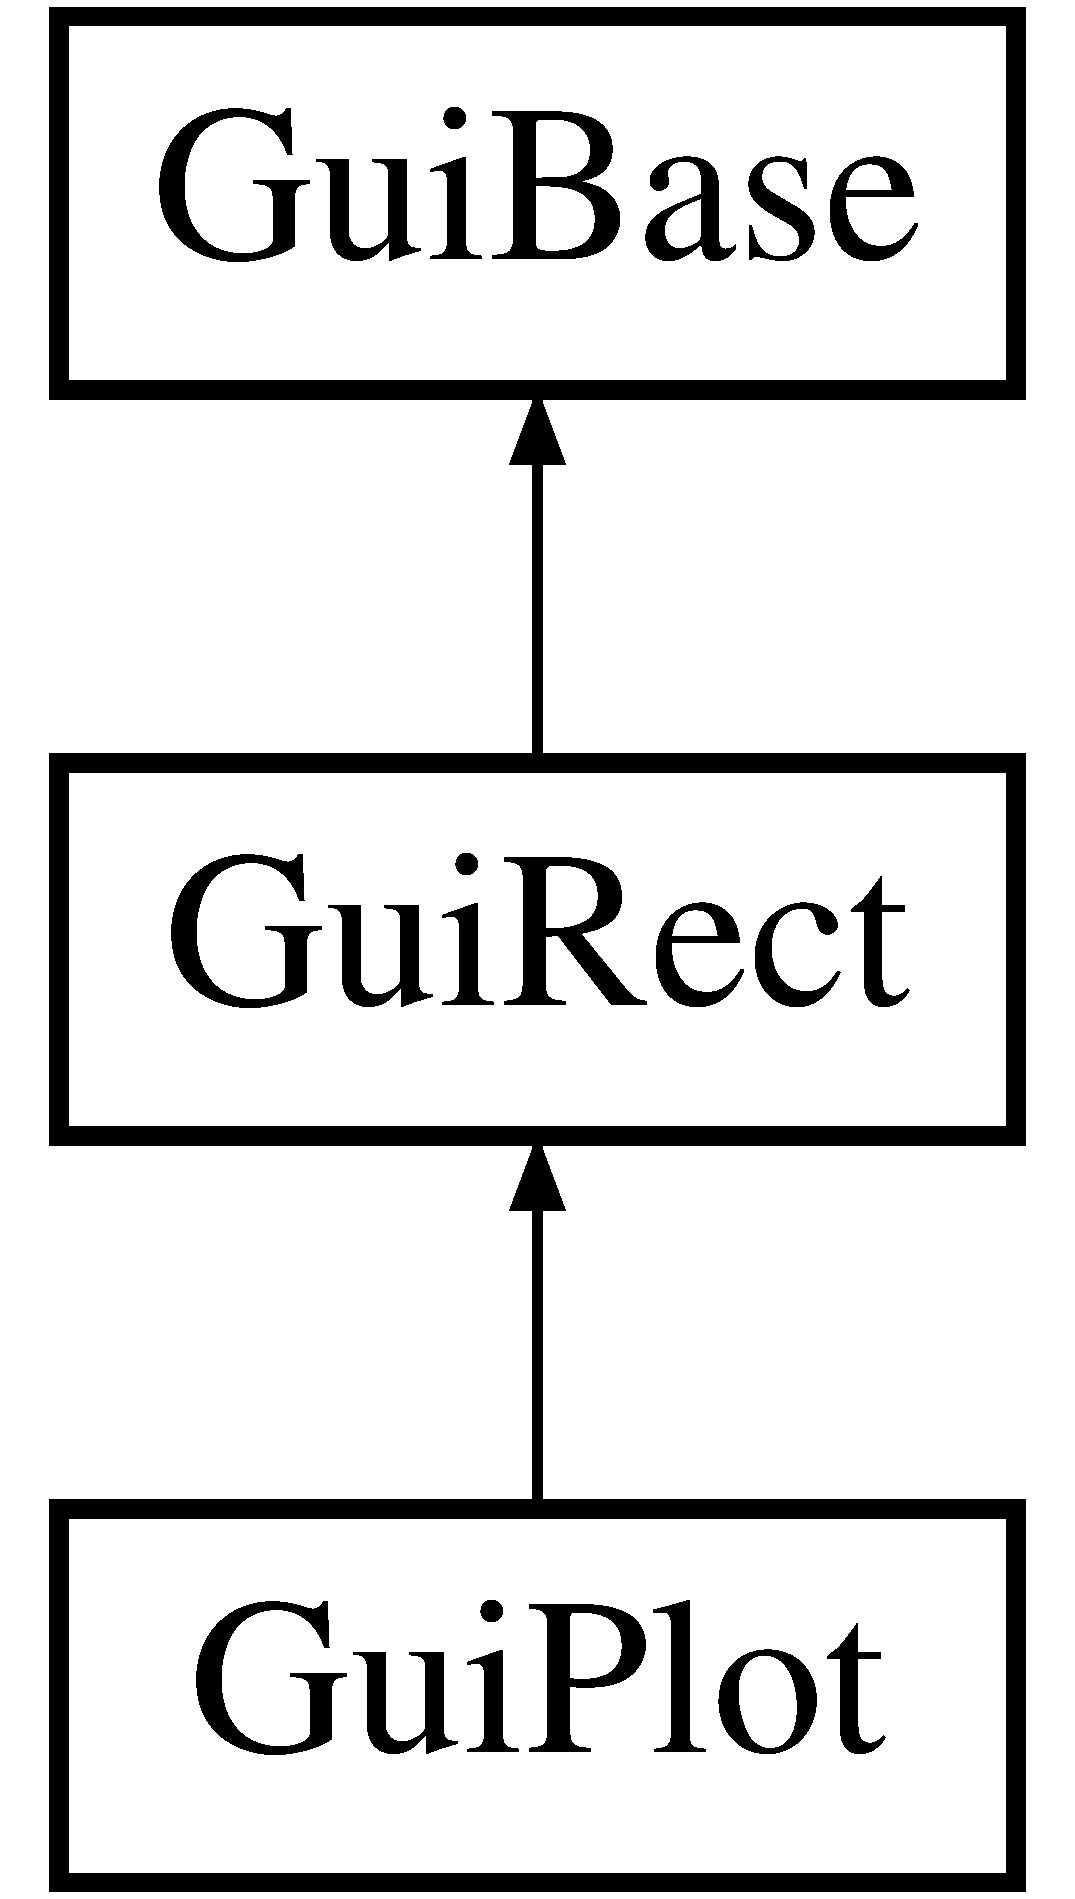
\includegraphics[height=3.000000cm]{class_gui_rect}
\end{center}
\end{figure}
\subsection*{Public Member Functions}
\begin{DoxyCompactItemize}
\item 
\hypertarget{class_gui_rect_a5bf3239a3fda5714e3b809fed8d2f18a}{\hyperlink{class_gui_rect_a5bf3239a3fda5714e3b809fed8d2f18a}{Gui\-Rect} ()}\label{class_gui_rect_a5bf3239a3fda5714e3b809fed8d2f18a}

\begin{DoxyCompactList}\small\item\em Default constructor. \end{DoxyCompactList}\item 
\hypertarget{class_gui_rect_a675b104d83a40f4451f39aca2da5963e}{virtual \hyperlink{class_gui_rect_a675b104d83a40f4451f39aca2da5963e}{$\sim$\-Gui\-Rect} ()}\label{class_gui_rect_a675b104d83a40f4451f39aca2da5963e}

\begin{DoxyCompactList}\small\item\em Virtual destructor. \end{DoxyCompactList}\item 
\hypertarget{class_gui_rect_abda31c93cd7ce05e2e90fa088e3cd7e2}{virtual void \hyperlink{class_gui_rect_abda31c93cd7ce05e2e90fa088e3cd7e2}{draw} ()}\label{class_gui_rect_abda31c93cd7ce05e2e90fa088e3cd7e2}

\begin{DoxyCompactList}\small\item\em An overloadable draw method. \end{DoxyCompactList}\item 
\hypertarget{class_gui_rect_aae1204fe60342bc98d23bb9313a84b4c}{void \hyperlink{class_gui_rect_aae1204fe60342bc98d23bb9313a84b4c}{set\-Fill\-Color} (const ci\-::\-Color\-A \&i\-Color)}\label{class_gui_rect_aae1204fe60342bc98d23bb9313a84b4c}

\begin{DoxyCompactList}\small\item\em Sets the rect's background color. \end{DoxyCompactList}\item 
\hypertarget{class_gui_rect_a6898af3268885b602a70b7fdb73bd317}{const ci\-::\-Color\-A \& \hyperlink{class_gui_rect_a6898af3268885b602a70b7fdb73bd317}{get\-Fill\-Color} () const }\label{class_gui_rect_a6898af3268885b602a70b7fdb73bd317}

\begin{DoxyCompactList}\small\item\em Returns the rect's background color. \end{DoxyCompactList}\item 
\hypertarget{class_gui_rect_a69059c87dd29c4867ac364a016c305ad}{void \hyperlink{class_gui_rect_a69059c87dd29c4867ac364a016c305ad}{set\-Stroke\-Color} (const ci\-::\-Color\-A \&i\-Color)}\label{class_gui_rect_a69059c87dd29c4867ac364a016c305ad}

\begin{DoxyCompactList}\small\item\em Sets the rect's border color. \end{DoxyCompactList}\item 
\hypertarget{class_gui_rect_abd68d08cff4e0a71e8122ce161e7ffb9}{const ci\-::\-Color\-A \& \hyperlink{class_gui_rect_abd68d08cff4e0a71e8122ce161e7ffb9}{get\-Stroke\-Color} () const }\label{class_gui_rect_abd68d08cff4e0a71e8122ce161e7ffb9}

\begin{DoxyCompactList}\small\item\em Returns the rect's border color. \end{DoxyCompactList}\item 
\hypertarget{class_gui_rect_a4aca606919a0081466c6fb77a018dda2}{void \hyperlink{class_gui_rect_a4aca606919a0081466c6fb77a018dda2}{set\-Stroke\-Weight} (const float \&i\-Weight)}\label{class_gui_rect_a4aca606919a0081466c6fb77a018dda2}

\begin{DoxyCompactList}\small\item\em Sets the rect's border width. \end{DoxyCompactList}\item 
\hypertarget{class_gui_rect_aba27ea56a68ecac460b4112c65055370}{const float \& \hyperlink{class_gui_rect_aba27ea56a68ecac460b4112c65055370}{get\-Stroke\-Weight} () const }\label{class_gui_rect_aba27ea56a68ecac460b4112c65055370}

\begin{DoxyCompactList}\small\item\em Returns the rect's border width. \end{DoxyCompactList}\end{DoxyCompactItemize}
\subsection*{Protected Attributes}
\begin{DoxyCompactItemize}
\item 
\hypertarget{class_gui_rect_a9c8999120a4fb5f654623195772a3988}{ci\-::\-Color\-A \hyperlink{class_gui_rect_a9c8999120a4fb5f654623195772a3988}{m\-Fill\-Color}}\label{class_gui_rect_a9c8999120a4fb5f654623195772a3988}

\begin{DoxyCompactList}\small\item\em The rect's background color. \end{DoxyCompactList}\item 
\hypertarget{class_gui_rect_a43b971fa2b7cf4afcfe476d693ba82a5}{ci\-::\-Color\-A \hyperlink{class_gui_rect_a43b971fa2b7cf4afcfe476d693ba82a5}{m\-Stroke\-Color}}\label{class_gui_rect_a43b971fa2b7cf4afcfe476d693ba82a5}

\begin{DoxyCompactList}\small\item\em The rect's border color. \end{DoxyCompactList}\item 
\hypertarget{class_gui_rect_a96f6a5cc17138bd803f22e4c4a180697}{float \hyperlink{class_gui_rect_a96f6a5cc17138bd803f22e4c4a180697}{m\-Stroke\-Weight}}\label{class_gui_rect_a96f6a5cc17138bd803f22e4c4a180697}

\begin{DoxyCompactList}\small\item\em The rect's border width. \end{DoxyCompactList}\end{DoxyCompactItemize}
\subsection*{Additional Inherited Members}


\subsection{Detailed Description}
A scenegraph node representing a rectangle. 

The documentation for this class was generated from the following files\-:\begin{DoxyCompactItemize}
\item 
/\-Users/pjh/\-Desktop/\-Work/\-Teaching/\-Creative\-Evolution\-Course/core/include/gui/Gui\-Rect.\-h\item 
/\-Users/pjh/\-Desktop/\-Work/\-Teaching/\-Creative\-Evolution\-Course/core/src/gui/Gui\-Rect.\-cpp\end{DoxyCompactItemize}

\hypertarget{class_gui_text}{\section{Gui\-Text Class Reference}
\label{class_gui_text}\index{Gui\-Text@{Gui\-Text}}
}


A scenegraph node representing a text label.  




{\ttfamily \#include $<$Gui\-Text.\-h$>$}

Inheritance diagram for Gui\-Text\-:\begin{figure}[H]
\begin{center}
\leavevmode
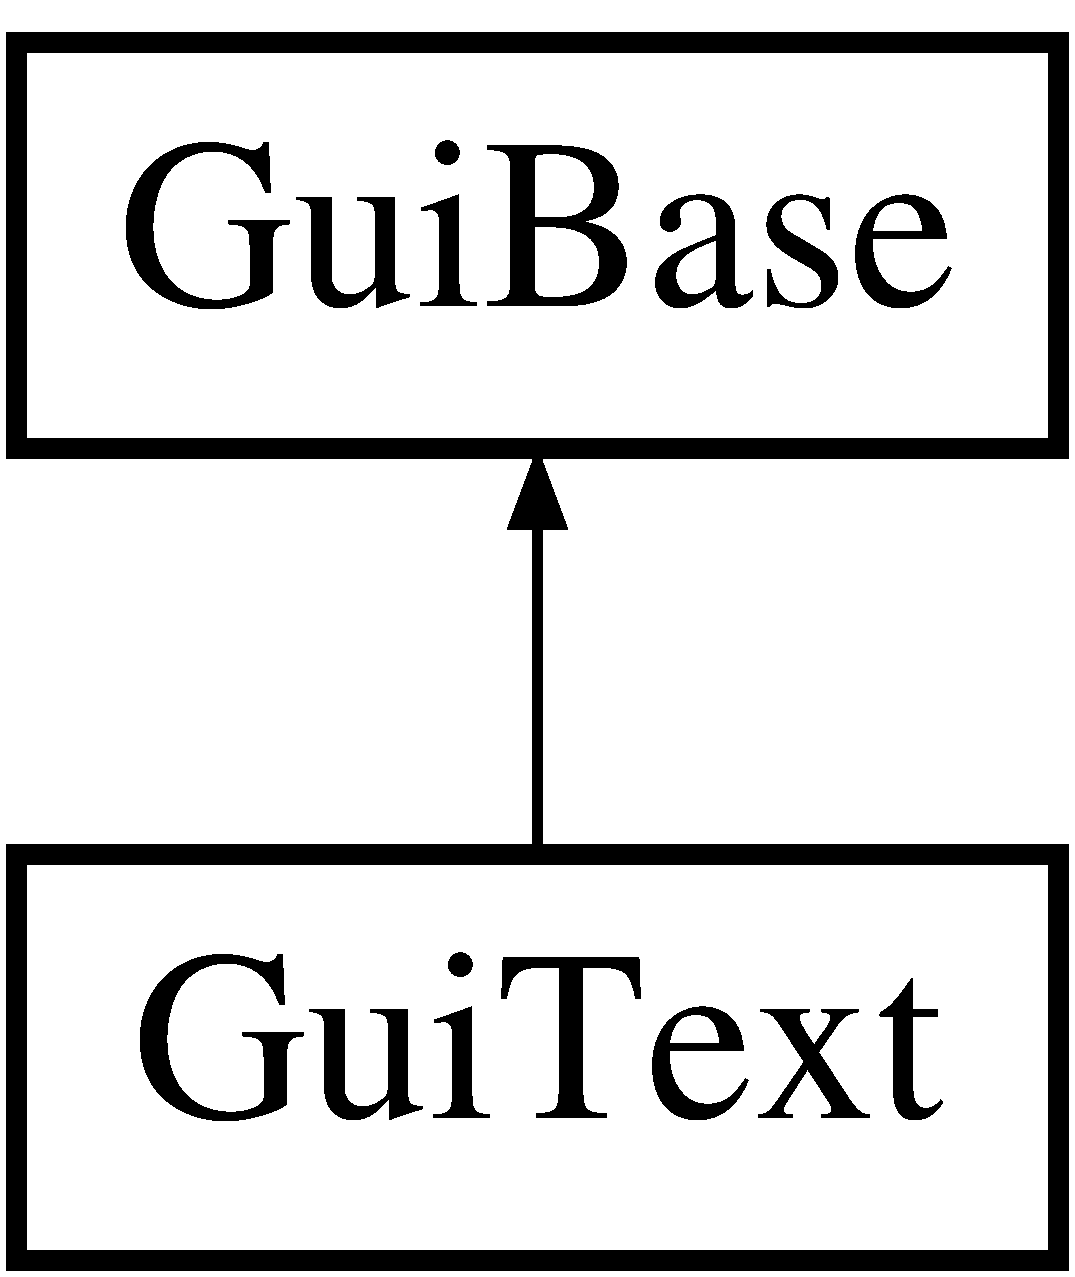
\includegraphics[height=2.000000cm]{class_gui_text}
\end{center}
\end{figure}
\subsection*{Public Member Functions}
\begin{DoxyCompactItemize}
\item 
\hypertarget{class_gui_text_a88cfe951bc47d61d292e13f9829bf1c2}{\hyperlink{class_gui_text_a88cfe951bc47d61d292e13f9829bf1c2}{Gui\-Text} (std\-::string i\-Text=\char`\"{}\char`\"{}, std\-::string i\-Font\-Name=\char`\"{}\char`\"{}, int i\-Font\-Size=12, Font\-Style i\-Style=Font\-Style\-::\-R\-E\-G\-U\-L\-A\-R, \hyperlink{class_font_suitcase}{Font\-Suitcase} $\ast$i\-Suitcase\-Ref=N\-U\-L\-L)}\label{class_gui_text_a88cfe951bc47d61d292e13f9829bf1c2}

\begin{DoxyCompactList}\small\item\em Basic constructor. \end{DoxyCompactList}\item 
\hypertarget{class_gui_text_a4fbdd1903c10906ac4b4ab5104d7599b}{virtual \hyperlink{class_gui_text_a4fbdd1903c10906ac4b4ab5104d7599b}{$\sim$\-Gui\-Text} ()}\label{class_gui_text_a4fbdd1903c10906ac4b4ab5104d7599b}

\begin{DoxyCompactList}\small\item\em Virtual destructor. \end{DoxyCompactList}\item 
\hypertarget{class_gui_text_a1bdcdc88b3b05523f54a5dd96146bfd0}{virtual void \hyperlink{class_gui_text_a1bdcdc88b3b05523f54a5dd96146bfd0}{draw} ()}\label{class_gui_text_a1bdcdc88b3b05523f54a5dd96146bfd0}

\begin{DoxyCompactList}\small\item\em An overloadable draw method. \end{DoxyCompactList}\item 
\hypertarget{class_gui_text_aa195f211e62bd4fcaa06a6ef129d4abc}{void \hyperlink{class_gui_text_aa195f211e62bd4fcaa06a6ef129d4abc}{set\-Text} (const std\-::string \&i\-Text)}\label{class_gui_text_aa195f211e62bd4fcaa06a6ef129d4abc}

\begin{DoxyCompactList}\small\item\em Sets the text label. \end{DoxyCompactList}\item 
\hypertarget{class_gui_text_a10261a9bbce64ec76b1b565f805df162}{const std\-::string \& \hyperlink{class_gui_text_a10261a9bbce64ec76b1b565f805df162}{get\-Text} () const }\label{class_gui_text_a10261a9bbce64ec76b1b565f805df162}

\begin{DoxyCompactList}\small\item\em Returns the text label. \end{DoxyCompactList}\item 
\hypertarget{class_gui_text_a9d48eb65fe6f5c3d022e40fba48b3898}{void \hyperlink{class_gui_text_a9d48eb65fe6f5c3d022e40fba48b3898}{set\-Text\-Color} (const ci\-::\-Color\-A \&i\-Color)}\label{class_gui_text_a9d48eb65fe6f5c3d022e40fba48b3898}

\begin{DoxyCompactList}\small\item\em Sets the text color. \end{DoxyCompactList}\item 
\hypertarget{class_gui_text_ac0701398fe08316be9e4b76248a9daf6}{const ci\-::\-Color\-A \& \hyperlink{class_gui_text_ac0701398fe08316be9e4b76248a9daf6}{get\-Text\-Color} () const }\label{class_gui_text_ac0701398fe08316be9e4b76248a9daf6}

\begin{DoxyCompactList}\small\item\em Returns the text color. \end{DoxyCompactList}\item 
\hypertarget{class_gui_text_a9ac5c71c03e77a9b1e074c2a5d0e4a6f}{void \hyperlink{class_gui_text_a9ac5c71c03e77a9b1e074c2a5d0e4a6f}{set\-Highlight\-Color} (const ci\-::\-Color\-A \&i\-Color)}\label{class_gui_text_a9ac5c71c03e77a9b1e074c2a5d0e4a6f}

\begin{DoxyCompactList}\small\item\em Sets the text highlight color. \end{DoxyCompactList}\item 
\hypertarget{class_gui_text_a3d07998b718c8dfccedb11b6bd449161}{const ci\-::\-Color\-A \& \hyperlink{class_gui_text_a3d07998b718c8dfccedb11b6bd449161}{get\-Highlight\-Color} () const }\label{class_gui_text_a3d07998b718c8dfccedb11b6bd449161}

\begin{DoxyCompactList}\small\item\em Returns the text highlight color. \end{DoxyCompactList}\item 
\hypertarget{class_gui_text_a3f696f0ea57bd16cae0f4c398720b7b5}{void \hyperlink{class_gui_text_a3f696f0ea57bd16cae0f4c398720b7b5}{set\-Guide\-Visibility} (const bool \&i\-Guides)}\label{class_gui_text_a3f696f0ea57bd16cae0f4c398720b7b5}

\begin{DoxyCompactList}\small\item\em Sets the visibility of the text guide lines. \end{DoxyCompactList}\item 
\hypertarget{class_gui_text_a06ec1fb156ab33fb94beeaa0d74e60c4}{const bool \& \hyperlink{class_gui_text_a06ec1fb156ab33fb94beeaa0d74e60c4}{get\-Guide\-Visibility} () const }\label{class_gui_text_a06ec1fb156ab33fb94beeaa0d74e60c4}

\begin{DoxyCompactList}\small\item\em Returns true if text guide lines are visible. \end{DoxyCompactList}\end{DoxyCompactItemize}
\subsection*{Protected Types}
\begin{DoxyCompactItemize}
\item 
\hypertarget{class_gui_text_aca27621ff95b564357e254f286050830}{typedef std\-::pair$<$ uint16\-\_\-t, \\*
ci\-::\-Vec2f $>$ \hyperlink{class_gui_text_aca27621ff95b564357e254f286050830}{Glyph\-Pair}}\label{class_gui_text_aca27621ff95b564357e254f286050830}

\begin{DoxyCompactList}\small\item\em A font glyph data item. \end{DoxyCompactList}\item 
\hypertarget{class_gui_text_add2a12dfdb7539d11f2df1961e0d48d8}{typedef std\-::vector$<$ \hyperlink{class_gui_text_aca27621ff95b564357e254f286050830}{Glyph\-Pair} $>$ \hyperlink{class_gui_text_add2a12dfdb7539d11f2df1961e0d48d8}{Glyph\-Vec}}\label{class_gui_text_add2a12dfdb7539d11f2df1961e0d48d8}

\begin{DoxyCompactList}\small\item\em A vector of font glyph data items. \end{DoxyCompactList}\item 
\hypertarget{class_gui_text_a054440052b7bdfce8730e2d886f6930a}{typedef Glyph\-Vec\-::iterator \hyperlink{class_gui_text_a054440052b7bdfce8730e2d886f6930a}{Glyph\-Vec\-Iter}}\label{class_gui_text_a054440052b7bdfce8730e2d886f6930a}

\begin{DoxyCompactList}\small\item\em An iterator type for a vector of font glyph data items. \end{DoxyCompactList}\item 
\hypertarget{class_gui_text_ab937be7c973011f0e263f8d603006767}{typedef Glyph\-Vec\-::reverse\-\_\-iterator \hyperlink{class_gui_text_ab937be7c973011f0e263f8d603006767}{Glyph\-Vec\-Riter}}\label{class_gui_text_ab937be7c973011f0e263f8d603006767}

\begin{DoxyCompactList}\small\item\em A reverse iterator type for a vector of font glyph data items. \end{DoxyCompactList}\item 
\hypertarget{class_gui_text_a29bb4d2e490498cc467836acd9f082d3}{typedef Glyph\-Vec\-::const\-\_\-iterator \hyperlink{class_gui_text_a29bb4d2e490498cc467836acd9f082d3}{Glyph\-Vec\-Citer}}\label{class_gui_text_a29bb4d2e490498cc467836acd9f082d3}

\begin{DoxyCompactList}\small\item\em A const iterator type for a vector of font glyph data items. \end{DoxyCompactList}\end{DoxyCompactItemize}
\subsection*{Protected Attributes}
\begin{DoxyCompactItemize}
\item 
\hypertarget{class_gui_text_a95494b51514f038ea1368ad385798c9b}{std\-::string \hyperlink{class_gui_text_a95494b51514f038ea1368ad385798c9b}{m\-Text}}\label{class_gui_text_a95494b51514f038ea1368ad385798c9b}

\begin{DoxyCompactList}\small\item\em The text label. \end{DoxyCompactList}\item 
\hypertarget{class_gui_text_aae0d080e6c974b0c72f56494e2932ab1}{ci\-::\-Color\-A \hyperlink{class_gui_text_aae0d080e6c974b0c72f56494e2932ab1}{m\-Text\-Color}}\label{class_gui_text_aae0d080e6c974b0c72f56494e2932ab1}

\begin{DoxyCompactList}\small\item\em The text color. \end{DoxyCompactList}\item 
\hypertarget{class_gui_text_a7ff0747e05176d28ed733706713f98ba}{ci\-::\-Color\-A \hyperlink{class_gui_text_a7ff0747e05176d28ed733706713f98ba}{m\-Highlight\-Color}}\label{class_gui_text_a7ff0747e05176d28ed733706713f98ba}

\begin{DoxyCompactList}\small\item\em The text highlight color. \end{DoxyCompactList}\item 
\hypertarget{class_gui_text_ae0e22d961bb923537ffc924e97b38915}{bool \hyperlink{class_gui_text_ae0e22d961bb923537ffc924e97b38915}{m\-Retina}}\label{class_gui_text_ae0e22d961bb923537ffc924e97b38915}

\begin{DoxyCompactList}\small\item\em Flags whether display is high-\/density. \end{DoxyCompactList}\item 
\hypertarget{class_gui_text_a468dfb3b1c78d9590d58009688a8214f}{bool \hyperlink{class_gui_text_a468dfb3b1c78d9590d58009688a8214f}{m\-Guides}}\label{class_gui_text_a468dfb3b1c78d9590d58009688a8214f}

\begin{DoxyCompactList}\small\item\em Flags whether text guides should be rendered. \end{DoxyCompactList}\item 
\hypertarget{class_gui_text_a508a0c19105346ba9a64b5117a4518a5}{\hyperlink{class_gui_text_add2a12dfdb7539d11f2df1961e0d48d8}{Glyph\-Vec} \hyperlink{class_gui_text_a508a0c19105346ba9a64b5117a4518a5}{m\-Glyphs}}\label{class_gui_text_a508a0c19105346ba9a64b5117a4518a5}

\begin{DoxyCompactList}\small\item\em Stores the text label's glyph placements. \end{DoxyCompactList}\item 
\hypertarget{class_gui_text_af11e0fe4d30f9ebd106b4fed42f1fa7f}{ci\-::gl\-::\-Texture\-Font\-Ref \hyperlink{class_gui_text_af11e0fe4d30f9ebd106b4fed42f1fa7f}{m\-Font\-Ref}}\label{class_gui_text_af11e0fe4d30f9ebd106b4fed42f1fa7f}

\begin{DoxyCompactList}\small\item\em A reference to the label's font. \end{DoxyCompactList}\item 
\hypertarget{class_gui_text_a90eb1509012b8ae37cffa32b404965e7}{ci\-::gl\-::\-Texture\-Font\-::\-Draw\-Options \hyperlink{class_gui_text_a90eb1509012b8ae37cffa32b404965e7}{m\-Font\-Options}}\label{class_gui_text_a90eb1509012b8ae37cffa32b404965e7}

\begin{DoxyCompactList}\small\item\em A reference to the label's font options. \end{DoxyCompactList}\end{DoxyCompactItemize}
\subsection*{Additional Inherited Members}


\subsection{Detailed Description}
A scenegraph node representing a text label. 

The documentation for this class was generated from the following files\-:\begin{DoxyCompactItemize}
\item 
/\-Users/pjh/\-Desktop/\-Work/\-Teaching/\-Creative\-Evolution\-Course/core/include/gui/Gui\-Text.\-h\item 
/\-Users/pjh/\-Desktop/\-Work/\-Teaching/\-Creative\-Evolution\-Course/core/src/gui/Gui\-Text.\-cpp\end{DoxyCompactItemize}

\hypertarget{class_plotter_data}{\section{Plotter\-Data Class Reference}
\label{class_plotter_data}\index{Plotter\-Data@{Plotter\-Data}}
}


Base class representing data to be plotted by \hyperlink{class_gui_plot}{Gui\-Plot}.  




{\ttfamily \#include $<$Gui\-Plot\-Data.\-h$>$}

Inheritance diagram for Plotter\-Data\-:\begin{figure}[H]
\begin{center}
\leavevmode
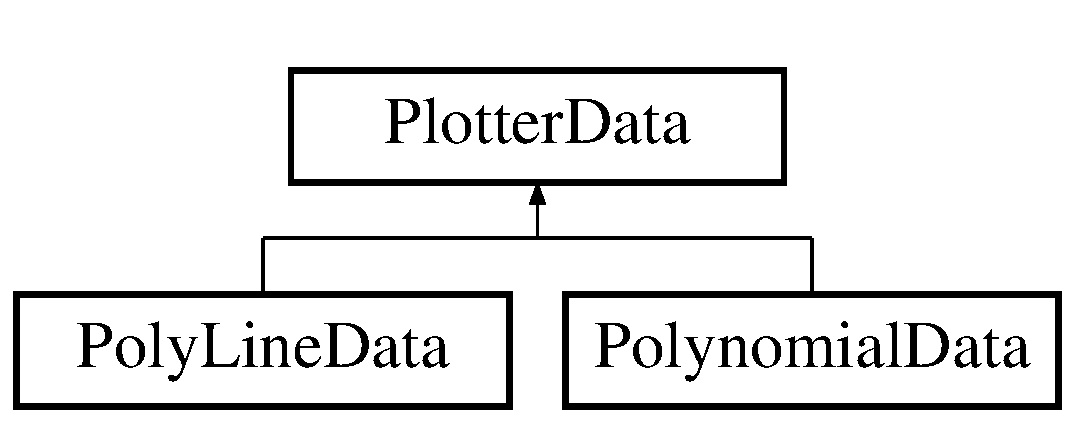
\includegraphics[height=2.000000cm]{class_plotter_data}
\end{center}
\end{figure}
\subsection*{Public Member Functions}
\begin{DoxyCompactItemize}
\item 
\hypertarget{class_plotter_data_a28cb319f221a9d910d3b589b3e9ed39c}{\hyperlink{class_plotter_data_a28cb319f221a9d910d3b589b3e9ed39c}{Plotter\-Data} (const ci\-::\-Color\-A \&i\-Color=ci\-::\-Color\-A\-::white(), const float \&i\-Stroke\-Weight=3.\-0)}\label{class_plotter_data_a28cb319f221a9d910d3b589b3e9ed39c}

\begin{DoxyCompactList}\small\item\em Basic constructor. \end{DoxyCompactList}\item 
\hypertarget{class_plotter_data_aa0843071635bab709d414e1c33896f82}{virtual \hyperlink{class_plotter_data_aa0843071635bab709d414e1c33896f82}{$\sim$\-Plotter\-Data} ()}\label{class_plotter_data_aa0843071635bab709d414e1c33896f82}

\begin{DoxyCompactList}\small\item\em Virtual destructor. \end{DoxyCompactList}\item 
\hypertarget{class_plotter_data_a00d9c9a8a11688d545b7f1457ce52191}{virtual \hyperlink{class_plotter_data}{Plotter\-Data} $\ast$ \hyperlink{class_plotter_data_a00d9c9a8a11688d545b7f1457ce52191}{clone} ()}\label{class_plotter_data_a00d9c9a8a11688d545b7f1457ce52191}

\begin{DoxyCompactList}\small\item\em Returns a clone of this item. \end{DoxyCompactList}\item 
\hypertarget{class_plotter_data_aa6970736c980752a277d80a27481cb4f}{virtual void \hyperlink{class_plotter_data_aa6970736c980752a277d80a27481cb4f}{draw} ()}\label{class_plotter_data_aa6970736c980752a277d80a27481cb4f}

\begin{DoxyCompactList}\small\item\em An overloadable draw method. \end{DoxyCompactList}\item 
\hypertarget{class_plotter_data_a3c424fcea7e761a4fe0d91975ebf6fae}{void \hyperlink{class_plotter_data_a3c424fcea7e761a4fe0d91975ebf6fae}{set\-Stroke\-Color} (const ci\-::\-Color\-A \&i\-Color)}\label{class_plotter_data_a3c424fcea7e761a4fe0d91975ebf6fae}

\begin{DoxyCompactList}\small\item\em Sets the data's stroke color. \end{DoxyCompactList}\item 
\hypertarget{class_plotter_data_af9b81e09f4cb47e0dab3b01f3f1b0e72}{const ci\-::\-Color\-A \& \hyperlink{class_plotter_data_af9b81e09f4cb47e0dab3b01f3f1b0e72}{get\-Stroke\-Color} () const }\label{class_plotter_data_af9b81e09f4cb47e0dab3b01f3f1b0e72}

\begin{DoxyCompactList}\small\item\em Returns the data's stroke color. \end{DoxyCompactList}\item 
\hypertarget{class_plotter_data_a94c7a633258a0ff47d1cf9652cc1c4e1}{void \hyperlink{class_plotter_data_a94c7a633258a0ff47d1cf9652cc1c4e1}{set\-Stroke\-Weight} (const float \&i\-Stroke\-Weight)}\label{class_plotter_data_a94c7a633258a0ff47d1cf9652cc1c4e1}

\begin{DoxyCompactList}\small\item\em Sets the data's stroke weight. \end{DoxyCompactList}\item 
\hypertarget{class_plotter_data_a5c27e760e3df81fdc27386eb3cca804c}{const float \& \hyperlink{class_plotter_data_a5c27e760e3df81fdc27386eb3cca804c}{get\-Stroke\-Weight} () const }\label{class_plotter_data_a5c27e760e3df81fdc27386eb3cca804c}

\begin{DoxyCompactList}\small\item\em Returns the data's stroke weight. \end{DoxyCompactList}\end{DoxyCompactItemize}
\subsection*{Protected Attributes}
\begin{DoxyCompactItemize}
\item 
\hypertarget{class_plotter_data_a27a91db0e47c5beb3e7d63c9fffc33f2}{ci\-::\-Color\-A \hyperlink{class_plotter_data_a27a91db0e47c5beb3e7d63c9fffc33f2}{m\-Color}}\label{class_plotter_data_a27a91db0e47c5beb3e7d63c9fffc33f2}

\begin{DoxyCompactList}\small\item\em The data's stroke color. \end{DoxyCompactList}\item 
\hypertarget{class_plotter_data_adcca0cf31a02559715f6202bc22f4bd3}{float \hyperlink{class_plotter_data_adcca0cf31a02559715f6202bc22f4bd3}{m\-Stroke\-Weight}}\label{class_plotter_data_adcca0cf31a02559715f6202bc22f4bd3}

\begin{DoxyCompactList}\small\item\em The data's stroke weight. \end{DoxyCompactList}\end{DoxyCompactItemize}


\subsection{Detailed Description}
Base class representing data to be plotted by \hyperlink{class_gui_plot}{Gui\-Plot}. 

The documentation for this class was generated from the following files\-:\begin{DoxyCompactItemize}
\item 
/\-Users/pjh/\-Desktop/\-Work/\-Teaching/\-Creative\-Evolution\-Course/core/include/gui/Gui\-Plot\-Data.\-h\item 
/\-Users/pjh/\-Desktop/\-Work/\-Teaching/\-Creative\-Evolution\-Course/core/src/gui/Gui\-Plot\-Data.\-cpp\end{DoxyCompactItemize}

\hypertarget{class_poly_line_data}{\section{Poly\-Line\-Data Class Reference}
\label{class_poly_line_data}\index{Poly\-Line\-Data@{Poly\-Line\-Data}}
}


Implements a subclass of \hyperlink{class_plotter_data}{Plotter\-Data} that stores ci\-::\-Poly\-Line2f data.  




{\ttfamily \#include $<$Gui\-Plot\-Data.\-h$>$}

Inheritance diagram for Poly\-Line\-Data\-:\begin{figure}[H]
\begin{center}
\leavevmode
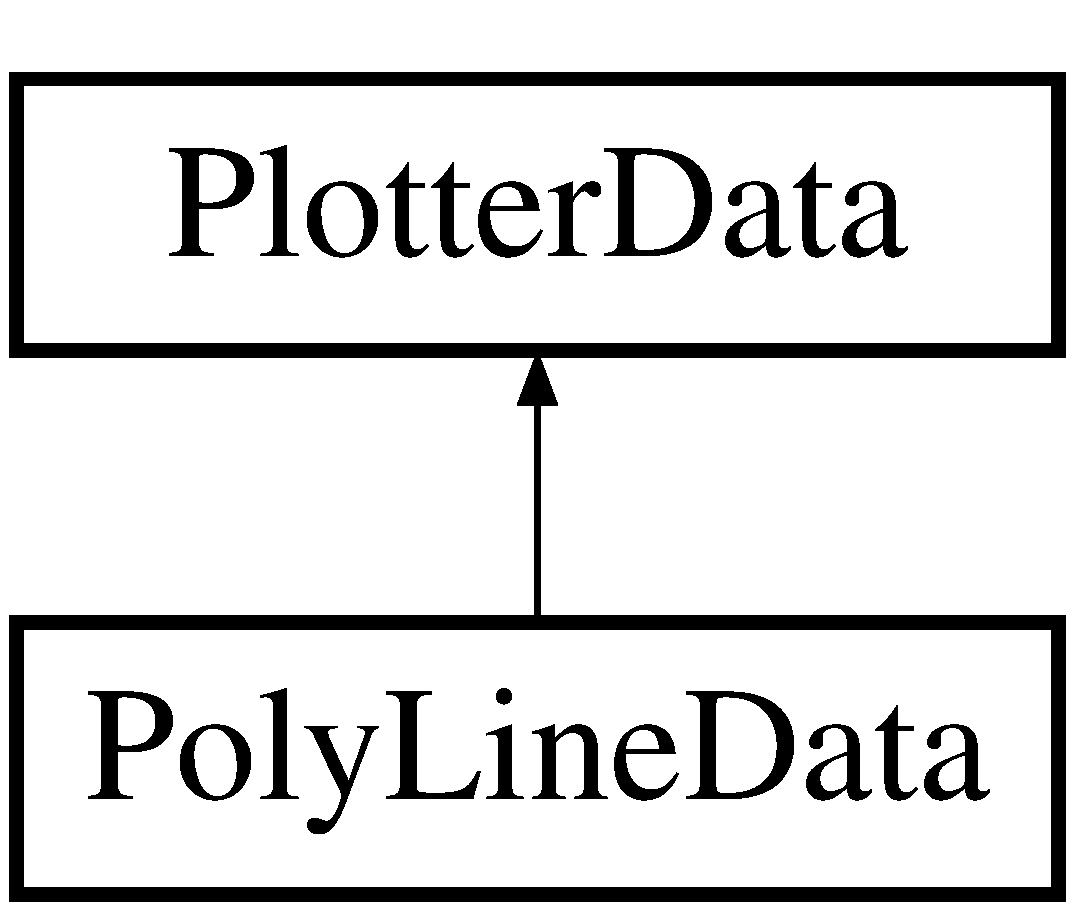
\includegraphics[height=2.000000cm]{class_poly_line_data}
\end{center}
\end{figure}
\subsection*{Public Member Functions}
\begin{DoxyCompactItemize}
\item 
\hypertarget{class_poly_line_data_a0abf8c7f195d3eb65ea07c675ea4a52f}{\hyperlink{class_poly_line_data_a0abf8c7f195d3eb65ea07c675ea4a52f}{Poly\-Line\-Data} ()}\label{class_poly_line_data_a0abf8c7f195d3eb65ea07c675ea4a52f}

\begin{DoxyCompactList}\small\item\em Default constructor. \end{DoxyCompactList}\item 
\hypertarget{class_poly_line_data_a5153e14acd22a7aa97e1bb37fd84dea7}{\hyperlink{class_poly_line_data_a5153e14acd22a7aa97e1bb37fd84dea7}{Poly\-Line\-Data} (const ci\-::\-Poly\-Line2f \&i\-Data, const ci\-::\-Color\-A \&i\-Color=ci\-::\-Color\-A\-::white(), const float \&i\-Stroke\-Weight=3.\-0)}\label{class_poly_line_data_a5153e14acd22a7aa97e1bb37fd84dea7}

\begin{DoxyCompactList}\small\item\em Basic constructor. \end{DoxyCompactList}\item 
\hypertarget{class_poly_line_data_a014782b028129033f7c4bc73990bd565}{virtual \hyperlink{class_poly_line_data_a014782b028129033f7c4bc73990bd565}{$\sim$\-Poly\-Line\-Data} ()}\label{class_poly_line_data_a014782b028129033f7c4bc73990bd565}

\begin{DoxyCompactList}\small\item\em Virtual destructor. \end{DoxyCompactList}\item 
\hypertarget{class_poly_line_data_abb4b40deb900d73bf5ff7e4775b207f8}{virtual \hyperlink{class_plotter_data}{Plotter\-Data} $\ast$ \hyperlink{class_poly_line_data_abb4b40deb900d73bf5ff7e4775b207f8}{clone} ()}\label{class_poly_line_data_abb4b40deb900d73bf5ff7e4775b207f8}

\begin{DoxyCompactList}\small\item\em Returns a clone of this item. \end{DoxyCompactList}\item 
\hypertarget{class_poly_line_data_a992ac9cb7fd7bfc38e5d7b1e727982ba}{virtual void \hyperlink{class_poly_line_data_a992ac9cb7fd7bfc38e5d7b1e727982ba}{draw} ()}\label{class_poly_line_data_a992ac9cb7fd7bfc38e5d7b1e727982ba}

\begin{DoxyCompactList}\small\item\em An overloadable draw method. \end{DoxyCompactList}\end{DoxyCompactItemize}
\subsection*{Protected Attributes}
\begin{DoxyCompactItemize}
\item 
\hypertarget{class_poly_line_data_a7d1bd43cc0baaacf38cfa9b9d538b01a}{ci\-::\-Poly\-Line2f \hyperlink{class_poly_line_data_a7d1bd43cc0baaacf38cfa9b9d538b01a}{m\-Data}}\label{class_poly_line_data_a7d1bd43cc0baaacf38cfa9b9d538b01a}

\begin{DoxyCompactList}\small\item\em The 2\-D Poly\-Line data. \end{DoxyCompactList}\end{DoxyCompactItemize}


\subsection{Detailed Description}
Implements a subclass of \hyperlink{class_plotter_data}{Plotter\-Data} that stores ci\-::\-Poly\-Line2f data. 

The documentation for this class was generated from the following files\-:\begin{DoxyCompactItemize}
\item 
/\-Users/pjh/\-Desktop/\-Work/\-Teaching/\-Creative\-Evolution\-Course/core/include/gui/Gui\-Plot\-Data.\-h\item 
/\-Users/pjh/\-Desktop/\-Work/\-Teaching/\-Creative\-Evolution\-Course/core/src/gui/Gui\-Plot\-Data.\-cpp\end{DoxyCompactItemize}

\hypertarget{class_polynomial_data}{\section{Polynomial\-Data Class Reference}
\label{class_polynomial_data}\index{Polynomial\-Data@{Polynomial\-Data}}
}


A class representing a polynomial function.  




{\ttfamily \#include $<$Polynomial\-Data.\-h$>$}

Inheritance diagram for Polynomial\-Data\-:\begin{figure}[H]
\begin{center}
\leavevmode
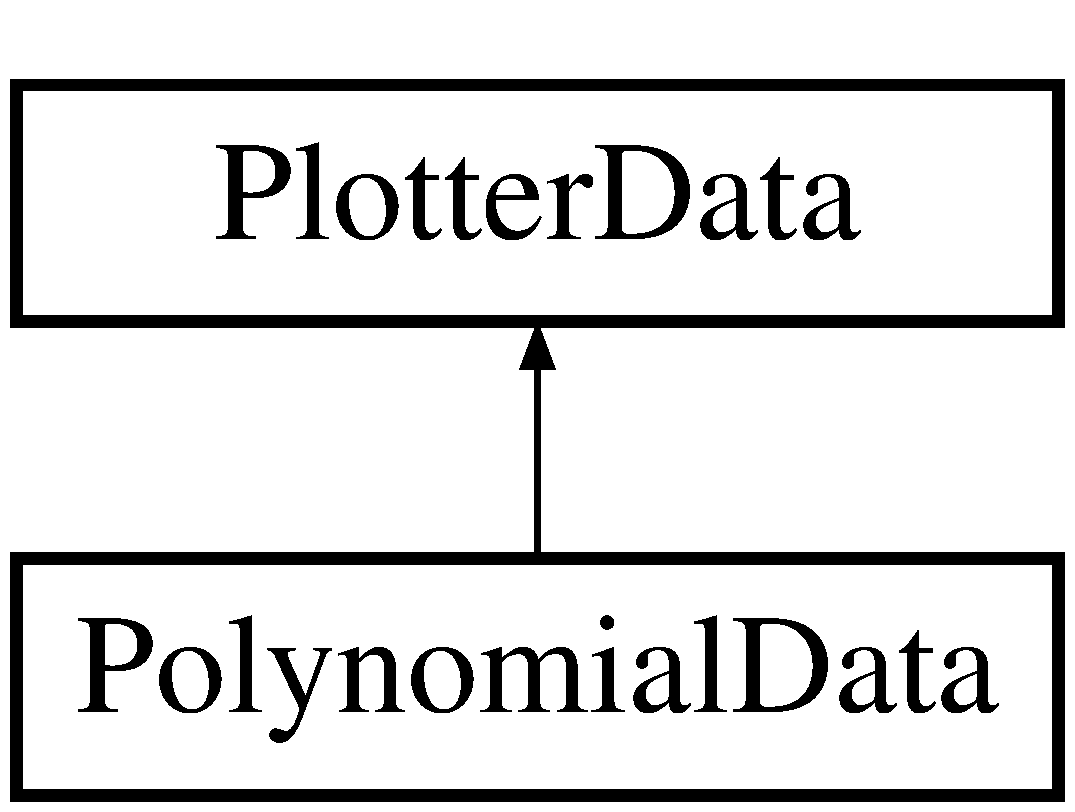
\includegraphics[height=2.000000cm]{class_polynomial_data}
\end{center}
\end{figure}
\subsection*{Public Types}
\begin{DoxyCompactItemize}
\item 
\hypertarget{class_polynomial_data_aa51d94a0bfb9c8a6a22b6f42bc876b86}{typedef std\-::pair$<$ float, float $>$ \hyperlink{class_polynomial_data_aa51d94a0bfb9c8a6a22b6f42bc876b86}{Component\-Pair}}\label{class_polynomial_data_aa51d94a0bfb9c8a6a22b6f42bc876b86}

\begin{DoxyCompactList}\small\item\em A $<$Coefficient,Exponent$>$ pair. \end{DoxyCompactList}\item 
\hypertarget{class_polynomial_data_aa29043ac29b9eefb530b6671be625814}{typedef std\-::vector\\*
$<$ \hyperlink{class_polynomial_data_aa51d94a0bfb9c8a6a22b6f42bc876b86}{Component\-Pair} $>$ \hyperlink{class_polynomial_data_aa29043ac29b9eefb530b6671be625814}{Component\-Vec}}\label{class_polynomial_data_aa29043ac29b9eefb530b6671be625814}

\begin{DoxyCompactList}\small\item\em A vector of $<$Coefficient,Exponent$>$ pairs. \end{DoxyCompactList}\item 
\hypertarget{class_polynomial_data_a5ae869760aeed6d622bd0229b8eb8d76}{typedef Component\-Vec\-::iterator \hyperlink{class_polynomial_data_a5ae869760aeed6d622bd0229b8eb8d76}{Component\-Vec\-Iter}}\label{class_polynomial_data_a5ae869760aeed6d622bd0229b8eb8d76}

\begin{DoxyCompactList}\small\item\em An iterator type for a vector of $<$Coefficient,Exponent$>$ pairs. \end{DoxyCompactList}\item 
\hypertarget{class_polynomial_data_a82be1374bb854aca018846d21094125e}{typedef \\*
Component\-Vec\-::reverse\-\_\-iterator \hyperlink{class_polynomial_data_a82be1374bb854aca018846d21094125e}{Component\-Vec\-Riter}}\label{class_polynomial_data_a82be1374bb854aca018846d21094125e}

\begin{DoxyCompactList}\small\item\em A reverse iterator type for a vector of $<$Coefficient,Exponent$>$ pairs. \end{DoxyCompactList}\item 
\hypertarget{class_polynomial_data_a7f77c4a643aa4b9fde19201969f8d787}{typedef \\*
Component\-Vec\-::const\-\_\-iterator \hyperlink{class_polynomial_data_a7f77c4a643aa4b9fde19201969f8d787}{Component\-Vec\-Citer}}\label{class_polynomial_data_a7f77c4a643aa4b9fde19201969f8d787}

\begin{DoxyCompactList}\small\item\em A const iterator type for a vector of $<$Coefficient,Exponent$>$ pairs. \end{DoxyCompactList}\end{DoxyCompactItemize}
\subsection*{Public Member Functions}
\begin{DoxyCompactItemize}
\item 
\hypertarget{class_polynomial_data_a2daf3355859ebb0886433ceab3276a7f}{\hyperlink{class_polynomial_data_a2daf3355859ebb0886433ceab3276a7f}{Polynomial\-Data} (const float \&i\-Param\-In=0.\-0, const float \&i\-Param\-Out=1.\-0, const bool \&i\-Draw\-Formula=true, const bool \&i\-Draw\-Deriv=true, const ci\-::\-Color\-A \&i\-Color=ci\-::\-Color\-A\-::white(), const float \&i\-Stroke\-Weight=3.\-0)}\label{class_polynomial_data_a2daf3355859ebb0886433ceab3276a7f}

\begin{DoxyCompactList}\small\item\em Basic Constructor. \end{DoxyCompactList}\item 
\hypertarget{class_polynomial_data_ae89bd56d2a8c7237b4688b4139f994cf}{virtual \hyperlink{class_polynomial_data_ae89bd56d2a8c7237b4688b4139f994cf}{$\sim$\-Polynomial\-Data} ()}\label{class_polynomial_data_ae89bd56d2a8c7237b4688b4139f994cf}

\begin{DoxyCompactList}\small\item\em Virtual destructor. \end{DoxyCompactList}\item 
\hypertarget{class_polynomial_data_ae6d60ae0791f477e4fd59d6694a38c2e}{virtual \hyperlink{class_plotter_data}{Plotter\-Data} $\ast$ \hyperlink{class_polynomial_data_ae6d60ae0791f477e4fd59d6694a38c2e}{clone} ()}\label{class_polynomial_data_ae6d60ae0791f477e4fd59d6694a38c2e}

\begin{DoxyCompactList}\small\item\em Returns a clone of this item. \end{DoxyCompactList}\item 
\hypertarget{class_polynomial_data_ad47bf7c086d64fef6c01e5542f47da79}{virtual void \hyperlink{class_polynomial_data_ad47bf7c086d64fef6c01e5542f47da79}{draw} ()}\label{class_polynomial_data_ad47bf7c086d64fef6c01e5542f47da79}

\begin{DoxyCompactList}\small\item\em An overloadable draw method. \end{DoxyCompactList}\item 
\hypertarget{class_polynomial_data_addcf3ab3c6147919c43f44dd9af97db7}{void \hyperlink{class_polynomial_data_addcf3ab3c6147919c43f44dd9af97db7}{set\-Draw\-Parameters} (const float \&i\-Param\-In, const float \&i\-Param\-Out, const bool \&i\-Draw\-Formula=true, const bool \&i\-Draw\-Deriv=true, const ci\-::\-Color\-A \&i\-Color=ci\-::\-Color\-A\-::white(), const float \&i\-Stroke\-Weight=3.\-0)}\label{class_polynomial_data_addcf3ab3c6147919c43f44dd9af97db7}

\begin{DoxyCompactList}\small\item\em Sets the parameter range for the drawing of the polynomial formula. \end{DoxyCompactList}\item 
\hypertarget{class_polynomial_data_a67c459e29c65ea79be11c6b9a209c6f8}{void \hyperlink{class_polynomial_data_a67c459e29c65ea79be11c6b9a209c6f8}{add\-Component} (const float \&i\-Coeff, const float \&i\-Expon)}\label{class_polynomial_data_a67c459e29c65ea79be11c6b9a209c6f8}

\begin{DoxyCompactList}\small\item\em Adds a component with the given coefficient and exponent values to the formula. \end{DoxyCompactList}\item 
\hypertarget{class_polynomial_data_ac2e4d723d0cde539326924933d34672a}{\hyperlink{class_polynomial_data_aa29043ac29b9eefb530b6671be625814}{Component\-Vec} \& \hyperlink{class_polynomial_data_ac2e4d723d0cde539326924933d34672a}{get\-Components} ()}\label{class_polynomial_data_ac2e4d723d0cde539326924933d34672a}

\begin{DoxyCompactList}\small\item\em Returns a reference to the components vector. \end{DoxyCompactList}\item 
\hypertarget{class_polynomial_data_ac34cf450bc6544e3b38aaeb3505f7f8d}{const \hyperlink{class_polynomial_data_aa29043ac29b9eefb530b6671be625814}{Component\-Vec} \& \hyperlink{class_polynomial_data_ac34cf450bc6544e3b38aaeb3505f7f8d}{get\-Components} () const }\label{class_polynomial_data_ac34cf450bc6544e3b38aaeb3505f7f8d}

\begin{DoxyCompactList}\small\item\em Returns a const reference to the components vector. \end{DoxyCompactList}\item 
\hypertarget{class_polynomial_data_ab04af5acc429792d65564a05b677aac1}{float \hyperlink{class_polynomial_data_ab04af5acc429792d65564a05b677aac1}{get\-Value} (const float \&i\-Param) const }\label{class_polynomial_data_ab04af5acc429792d65564a05b677aac1}

\begin{DoxyCompactList}\small\item\em Computes the output value for a given input. \end{DoxyCompactList}\item 
\hypertarget{class_polynomial_data_a8a5e239056596df41ff680e553b04f78}{float \hyperlink{class_polynomial_data_a8a5e239056596df41ff680e553b04f78}{get\-Derivative\-Value} (const float \&i\-Param) const }\label{class_polynomial_data_a8a5e239056596df41ff680e553b04f78}

\begin{DoxyCompactList}\small\item\em Computes the derivative of the output value for a given input. \end{DoxyCompactList}\item 
\hypertarget{class_polynomial_data_a5ef4f78a9e1e486ada0c97876a81c346}{std\-::string \hyperlink{class_polynomial_data_a5ef4f78a9e1e486ada0c97876a81c346}{get\-Formula\-String} () const }\label{class_polynomial_data_a5ef4f78a9e1e486ada0c97876a81c346}

\begin{DoxyCompactList}\small\item\em Returns a textual representation of the formula. \end{DoxyCompactList}\item 
\hypertarget{class_polynomial_data_a245b3a198847a4f393e9017f428bb52b}{std\-::string \hyperlink{class_polynomial_data_a245b3a198847a4f393e9017f428bb52b}{get\-Derivative\-Formula\-String} () const }\label{class_polynomial_data_a245b3a198847a4f393e9017f428bb52b}

\begin{DoxyCompactList}\small\item\em Returns a textual representation of the derivative formula. \end{DoxyCompactList}\end{DoxyCompactItemize}
\subsection*{Protected Attributes}
\begin{DoxyCompactItemize}
\item 
\hypertarget{class_polynomial_data_aa2a30c7dffdb123c572ad60b3af70f51}{\hyperlink{class_polynomial_data_aa29043ac29b9eefb530b6671be625814}{Component\-Vec} \hyperlink{class_polynomial_data_aa2a30c7dffdb123c572ad60b3af70f51}{m\-Components}}\label{class_polynomial_data_aa2a30c7dffdb123c572ad60b3af70f51}

\begin{DoxyCompactList}\small\item\em The formula's components. \end{DoxyCompactList}\item 
\hypertarget{class_polynomial_data_af989f08bb8d62cd2ed704eb44f9b3adf}{size\-\_\-t \hyperlink{class_polynomial_data_af989f08bb8d62cd2ed704eb44f9b3adf}{m\-Draw\-Samples}}\label{class_polynomial_data_af989f08bb8d62cd2ed704eb44f9b3adf}

\begin{DoxyCompactList}\small\item\em The number of samples to be plotted. \end{DoxyCompactList}\item 
\hypertarget{class_polynomial_data_a5190d5ec249c05a426080991d357e40f}{float \hyperlink{class_polynomial_data_a5190d5ec249c05a426080991d357e40f}{m\-Draw\-Range\-In}}\label{class_polynomial_data_a5190d5ec249c05a426080991d357e40f}

\begin{DoxyCompactList}\small\item\em The beginning of the param range. \end{DoxyCompactList}\item 
\hypertarget{class_polynomial_data_abff5e934de5f2cc78876e2da2f0867f1}{float \hyperlink{class_polynomial_data_abff5e934de5f2cc78876e2da2f0867f1}{m\-Draw\-Range\-Out}}\label{class_polynomial_data_abff5e934de5f2cc78876e2da2f0867f1}

\begin{DoxyCompactList}\small\item\em The end of the param range. \end{DoxyCompactList}\item 
\hypertarget{class_polynomial_data_ace6de172472e4b95b76d13dd21f999da}{bool \hyperlink{class_polynomial_data_ace6de172472e4b95b76d13dd21f999da}{m\-Draw\-Formula}}\label{class_polynomial_data_ace6de172472e4b95b76d13dd21f999da}

\begin{DoxyCompactList}\small\item\em Flags whether formula data should be drawn. \end{DoxyCompactList}\item 
\hypertarget{class_polynomial_data_a665a958ff21bf9969f842eb95818e891}{bool \hyperlink{class_polynomial_data_a665a958ff21bf9969f842eb95818e891}{m\-Draw\-Deriv}}\label{class_polynomial_data_a665a958ff21bf9969f842eb95818e891}

\begin{DoxyCompactList}\small\item\em Flags whether derivative data should be drawn. \end{DoxyCompactList}\item 
\hypertarget{class_polynomial_data_a278f68eb6b129f4635dd5bdbeef62ff6}{bool \hyperlink{class_polynomial_data_a278f68eb6b129f4635dd5bdbeef62ff6}{m\-Dirty}}\label{class_polynomial_data_a278f68eb6b129f4635dd5bdbeef62ff6}

\begin{DoxyCompactList}\small\item\em Flags whether raster data needs updating. \end{DoxyCompactList}\end{DoxyCompactItemize}


\subsection{Detailed Description}
A class representing a polynomial function. 

The documentation for this class was generated from the following files\-:\begin{DoxyCompactItemize}
\item 
/\-Users/pjh/\-Desktop/\-Work/\-Teaching/\-Creative\-Evolution\-Course/core/include/genetic/Polynomial\-Data.\-h\item 
/\-Users/pjh/\-Desktop/\-Work/\-Teaching/\-Creative\-Evolution\-Course/core/src/genetic/Polynomial\-Data.\-cpp\end{DoxyCompactItemize}

\hypertarget{class_polynomial_population}{\section{Polynomial\-Population Class Reference}
\label{class_polynomial_population}\index{Polynomial\-Population@{Polynomial\-Population}}
}


A population container and evolutionary process facilitation class for polynomial data and assertions.  




{\ttfamily \#include $<$Polynomial\-Population.\-h$>$}

\subsection*{Public Types}
\begin{DoxyCompactItemize}
\item 
\hypertarget{class_polynomial_population_a568edac365b311b32b0cd1615b75a961}{typedef std\-::shared\-\_\-ptr\\*
$<$ std\-::thread $>$ \hyperlink{class_polynomial_population_a568edac365b311b32b0cd1615b75a961}{Thread\-Ref}}\label{class_polynomial_population_a568edac365b311b32b0cd1615b75a961}

\begin{DoxyCompactList}\small\item\em A shared\-\_\-ptr thread wrapper type. \end{DoxyCompactList}\item 
\hypertarget{class_polynomial_population_a04e8d961feacdb2b80c3320c65c85d5b}{typedef \\*
ci\-::\-Concurrent\-Circular\-Buffer\\*
$<$ Polynomial\-Data\-Ref $>$ \hyperlink{class_polynomial_population_a04e8d961feacdb2b80c3320c65c85d5b}{Buffer}}\label{class_polynomial_population_a04e8d961feacdb2b80c3320c65c85d5b}

\begin{DoxyCompactList}\small\item\em A concurrent buffer type. \end{DoxyCompactList}\end{DoxyCompactItemize}
\subsection*{Public Member Functions}
\begin{DoxyCompactItemize}
\item 
\hypertarget{class_polynomial_population_aabdc5815c2f71683f8946503a91845bc}{\hyperlink{class_polynomial_population_aabdc5815c2f71683f8946503a91845bc}{Polynomial\-Population} (const \hyperlink{class_assertion_group}{Assertion\-Group} \&i\-Assertion\-Group, const size\-\_\-t \&i\-Population\-Size, const size\-\_\-t \&i\-Max\-Generation\-Count, const float \&i\-Mutation\-Rate, const float \&i\-Perfect\-Score=1e12)}\label{class_polynomial_population_aabdc5815c2f71683f8946503a91845bc}

\begin{DoxyCompactList}\small\item\em Basic constructor. \end{DoxyCompactList}\item 
\hypertarget{class_polynomial_population_a02b52e7f55d3c0265baba5c0b8df7c5d}{\hyperlink{class_polynomial_population_a02b52e7f55d3c0265baba5c0b8df7c5d}{$\sim$\-Polynomial\-Population} ()}\label{class_polynomial_population_a02b52e7f55d3c0265baba5c0b8df7c5d}

\begin{DoxyCompactList}\small\item\em Destructor. \end{DoxyCompactList}\item 
\hypertarget{class_polynomial_population_af42a7bf4c36d5adf25a12acc29a1b7b1}{bool \hyperlink{class_polynomial_population_af42a7bf4c36d5adf25a12acc29a1b7b1}{has\-Update} ()}\label{class_polynomial_population_af42a7bf4c36d5adf25a12acc29a1b7b1}

\begin{DoxyCompactList}\small\item\em Returns true if the internal buffer contains at least one item. \end{DoxyCompactList}\item 
\hypertarget{class_polynomial_population_a3a5efce92419c5da88f2199abe8c4c16}{Polynomial\-Data\-Ref \hyperlink{class_polynomial_population_a3a5efce92419c5da88f2199abe8c4c16}{get\-Update} ()}\label{class_polynomial_population_a3a5efce92419c5da88f2199abe8c4c16}

\begin{DoxyCompactList}\small\item\em Pops an item from the internal buffer and returns it in a thread-\/safe manner. \end{DoxyCompactList}\end{DoxyCompactItemize}


\subsection{Detailed Description}
A population container and evolutionary process facilitation class for polynomial data and assertions. 

The documentation for this class was generated from the following files\-:\begin{DoxyCompactItemize}
\item 
/\-Users/pjh/\-Desktop/\-Work/\-Teaching/\-Creative\-Evolution\-Course/core/include/genetic/Polynomial\-Population.\-h\item 
/\-Users/pjh/\-Desktop/\-Work/\-Teaching/\-Creative\-Evolution\-Course/core/src/genetic/Polynomial\-Population.\-cpp\end{DoxyCompactItemize}

\addcontentsline{toc}{part}{Index}
\printindex
\end{document}
